\documentclass{article}
\usepackage[utf8]{inputenc}
\usepackage[dutch]{babel}
\usepackage{amsthm}
\usepackage{amssymb}
\usepackage{mathtools}
\usepackage[margin=3cm]{geometry}
\usepackage[hidelinks]{hyperref}

\usepackage{fancyhdr}

\pagestyle{fancy}
\fancyhf{}
\lhead{\rightmark}
\rhead{Jonas van der Schaaf}
\fancyfoot[C]{\thepage}

\newcommand{\defeq}{\vcentcolon=}
\newcommand{\eqdef}{=\vcentcolon}
\newcommand{\bq}{``}
\newcommand{\eq}{''}
\renewcommand{\lim}[2]{\underset{#1\to#2}{\text{lim}}}
\newcommand{\uplim}[2]{\underset{#1\uparrow#2}{\text{lim}}\:}
\newcommand{\downlim}[2]{\underset{#1\downarrow#2}{\text{lim}}\:}
\newcommand{\liminfty}[1]{\lim{#1}{\infty}}
\newcommand{\limneginfty}[1]{\lim{#1}{-\infty}}
\newcommand{\sequenceset}{\mathbb{R}^{\mathbb{N}}}
\newcommand{\secnewpage}[1]{\newpage\section{#1}}
\newcommand{\subsecnewpage}[1]{\newpage\subsection{#1}}

\title{Samenvatting Analyse op de Lijn}
\author{Jonas van der Schaaf}

\begin{document}

\maketitle

\tableofcontents

\newpage

<<<<<<< HEAD
\section{Introductie}

<<<<<<< HEAD
\subsection{De verzameling $\mathbb{R}$}
\paragraph{Algebraïsche eigenschappen}De verzameling breuken $\mathbb{Q}$ heeft de volgende algebraïsche eigenschappen:
\begin{itemize}
    \setlength\itemsep{0em}
    \item[\textbf{A1.}] $a+(b+c)=(a+b)+c$ voor elke $a,b,c\in\mathbb{Q}$.
    \item[\textbf{A2.}] $a+b=b+a$ voor alle $a,b\in\mathbb{Q}$.
    \item[\textbf{A3.}] $a+0=0$ voor alle $a\in\mathbb{Q}$.
    \item[\textbf{A4.}] Voor elke $a\in\mathbb{Q}$ is er een $-a\in\mathbb{Q}$ zodat $a+(-a)=0$
    \item[\textbf{M1.}] $a(bc)=(ab)c$ voor elke $a,b,c\in\mathbb{Q}$.
    \item[\textbf{M2.}] $ab=ba$ voor alle $a,b\in\mathbb{Q}$.
    \item[\textbf{M3.}] $a\cdot1=a$ voor alle $a\in\mathbb{Q}$.
    \item[\textbf{M4.}] Voor elke $a\in\mathbb{Q}$ met $a\neq0$ is er een $a^{-1}\in\mathbb{Q}$ zodat $a \cdot a^{-1} = 1$
\end{itemize}
De eigenschappen \textbf{A1} en \textbf{M1} zijn de \textit{associatieve} eigenschappen van $+$ en $\cdot$ en de eigenschappen \textbf{A2} en \textbf{M2} zijn de \textit{commutatieve} eigenschappen van $+$ en $\cdot$.

\subparagraph{Consequenties van de veld eigenschappen} De volgende eigenschappen volgen uit de algebraïsche eigenschappen van $\mathbb{Q}$:

\begin{enumerate}
    \setlength\itemsep{0em}
    \item Als $a+c=b+c$ dan geldt dat $a=b$.
    \item $a\cdot0=0$ voor alle $a\in\mathbb{Q}$.
    \item $(-a)b=-ab$ voor alle $a,b\in\mathbb{Q}$.
    \item $(-a)(-b)=ab$ voor alle $a,b\in\mathbb{Q}$.
    \item Als $ac=bc$ en $c\neq0$ dan $a=b$.
    \item Als $ab=0$ dan geldt dat $a=0$ of $b=0$.
\end{enumerate}
\textit{De bewijzen van deze stellingen staan op pagina 16 van het boek.}

\paragraph{Ordening}Ook heeft $\mathbb{Q}$ een ordening \bq$\leq$\eq die aan de volgende eigenschappen voldoet:
\begin{itemize}
    \setlength\itemsep{0em}
    \item[\textbf{O1.}] Als $a,b\in\mathbb{Q}$ dan geldt dat $a \leq b$ of $b \leq a$.
    \item[\textbf{O2.}] Als $a \leq b$ en $b \leq a$ dan $a=b$.
    \item[\textbf{O3.}] Als $a \leq b$ en $b \leq c$ dan $a \leq c$.
    \item[\textbf{O4.}] Als $a \leq b$ dan geldt ook dat $a+c \leq b+c$
    \item[\textbf{O5.}] Als $a \leq b$ en $c \geq 0$, dan ook $ac \leq bc$.
\end{itemize}
De eigenschap \textbf{O3} heet de \textit{transitieve} eigenschap. Een veld met een ordening die voldoet aan \textbf{O1} tot en met \textbf{O5} heet een geordend veld.

\subparagraph{Consequenties van de ordening ''$\leq$''}
\begin{enumerate}
    \setlength\itemsep{0em}
    \item Als $a \leq b$ dan $-b \leq -a$.
    \item Als $a \leq b$ en $c\leq0$ dan $bc \leq ac$.
    \item Als $0 \leq a$ en $0 \leq b$ dan $0 \leq ab$.
    \item $0 \leq a^{2}$ voor elke $a\in\mathbb{Q}$.
    \item $0<1$.
    \item Als $0 < a$ dan ook $0 < a^{-1}$.
    \item Als $0<a<b$ dan geldt $0<b^{-1}<a^{-1}$.
\end{enumerate}
\textit{Dit wordt bewezen op pagina 16-17 van het boek.}

\paragraph{Absolute waarde} De absolute waarde is gedefinieerd als volgt:
$$
|a|\defeq
\begin{cases}
    a & \text{als } a\geq 0\\
    -a & \text{als } a<0
\end{cases}
$$
\subparagraph{Stellingen over de absolute waarde} De volgende stellingen over de absolute waarde zijn waar:
\begin{enumerate}
    \setlength\itemsep{0em}
    \item $|a|\geq0$.
    \item $|ab|=|a|\cdot|b|$.
    \item $|a+b|\leq|a|+|b|$.
\end{enumerate}
\textit{Dit wordt bewezen op pagina 17-18 van het boek.}

\paragraph{Afstand} De afstand tussen twee getallen $a,b$ is de $\text{dist}(a,b)$ wat gedefiniëerd is als:
$$\text{dist}(a,b)\defeq|a-b|$$
\paragraph{Stellingen over de afstand} De volgende stelling over afstand is waar:

\subparagraph{Afstand tussen de som van getallen} $\text{dist}(a,c)\leq\text{dist}(a,b)+\text{dist}(b,c)$.

\textit{Dit wordt bewezen op pagina 18 van het boek.}

\paragraph{Stellingen uit opgaven} De volgende handige stellingen worden bewezen in een opgave uit paragraaf $3$:

\subparagraph{Opgave 3.5a} Voor elke $a,b\in\mathbb{R}$ geldt dat $|b| \leq a$ dan en slechts dan als $-a \leq b \leq a$.

\subparagraph{Opgave 3.5b} Voor elke $a,b\in\mathbb{R}$ geldt dat $||b|-|a|| \leq |b-a|$.

\subparagraph{Opgave 3.6b} Laat $a_{1},a_{2},...,a_{n}\in\mathbb{R}$, dan geldt dat $|\sum_{i=1}^{n}a_{i}|\leq\sum_{i=1}^{n}|a_{i}|$
\subsection{De compleetheid van \texorpdfstring{$\mathbb{R}$}{R}}

\paragraph{Maxima en minima} Van een verzameling $S\subseteq\mathbb{R}$ zijn het maximum en minimum als volgt gedefiniëerd:
\subparagraph{Maximum} $s_{0} = \text{max}(S)$ dan en slechts dan als voor elke $s \in S$ geldt dat $s \leq s_{0}$ en $s_{0} \in S$.
\subparagraph{Minimum}$s_{0} = \text{min}(S)$ dan en slechts dan als voor elke $s \in S$ geldt dat $s \geq s_{0}$ en $s_{0} \in S$.

\paragraph{Intervallen} Een interval is een speciaal soort deelverzameling van $\mathbb{R}$, er zijn 4 verschillende intervallen:
\begin{itemize}
    \setlength\itemsep{0em}
    \item $[a,b]\defeq\{x\in\mathbb{R}:a \leq x \leq b\}$ dit heet een gesloten interval. $\text{min}([a,b])=a$ en $\text{max}([a,b])=b$.
    \item $[a,b)\defeq\{x\in\mathbb{R}:a \leq x < b\}$ dit heet een half gesloten interval. $\text{min}([a,b))=a$ en $\text{max}([a,b))$ bestaat niet.
    \item $(a,b]\defeq\{x\in\mathbb{R}:a < x \leq b\}$ dit heet een half gesloten interval. $\text{min}((a,b])=a$ en $\text{max}((a,b])$ bestaat niet.
    \item $(a,b)\defeq\{x\in\mathbb{R}:a < x < b\}$ dit heet een open interval. $\text{min}((a,b))$ bestaat niet en $\text{max}((a,b))$ bestaat niet.
\end{itemize}

\paragraph{Boven- en ondergrenzen} Boven- en ondergrenzen zijn als volgt gedefiniëerd: Laat $S\subseteq\mathbb{R}$ dan geldt

\subparagraph{Bovengrens} Een getal $M$ is een bovengrens van $S$ als voor elke $s \in S$ geldt dat $s \leq M$. Als een verzameling een bovengrens heeft dan heet die verzameling boven begrensd.

\subparagraph{Ondergrens} Een getal $m$ is een ondergrens van $S$ als voor elke $s \in S$ geldt dat $s \geq m$. Als een verzameling een ondergrens heeft dan heet die verzameling onder begrensd.

\paragraph{Stellingen over boven- en ondergrenzen} De volgende stelling wordt gegeven over bovengrenzen:

\subparagraph{Intervallen en begrenzingen} Als $S$ boven en beneden begrensd is, dan zijn er twee getallen $m,M\in\mathbb{R}$ zodat $S\subseteq [m,M]$.

\paragraph{Suprema en infima} Het supremum en infimum van een verzameling zijn als volgt gedefiniëerd:

\subparagraph{Supremum} $M=\text{sup}(S)$ dan en slechts dan als voor elke $s \in S$ geldt dat $s \leq M$ en voor elke $M_{1}<M$ geldt dat er een $s \in S$ is zodat $M_{1}<s$. Dan is $M$ de kleinste bovengrens van $S$.

\subparagraph{Infimum} $m=\text{inf}(S)$ dan en slechts dan als voor elke $s \in S$ geldt dat $m \geq s$ en voor elke $m>m_{1}$ geldt dat er een $s \in S$ waarvoor geldt dat $s<m$. Dan is $m$ de grootste ondergrens van $S$.

\paragraph{Stellingen} In paragraaf 4 van hoofdstuk 1 staan de volgende stellingen:

\subparagraph{Volledigheidsaxioma van $\mathbb{R}$} Het volledigheidsaxioma luidt als volgt: Voor elke $S\subseteq\mathbb{R}$ met $S\neq\emptyset$ met een bovengrens is er een $M\in\mathbb{R}$ zodat $M=\text{sup}(S)$. \textit{Dit is een axioma, er is geen bewijs.}

\subparagraph{``Omgekeerde'' volledigheids \bq axioma\eq} Voor elke $S\in\mathbb{R}$ met $S\neq\emptyset$ met een ondergrens is er een $m\in\mathbb{R}$ zodat $m=\text{inf}(S)$. Het is geen echt axioma want het volgt uit het volledigheidsaxioma. \textit{Het bewijs staat op pagina 24-25 van het boek.}

\subparagraph{Archimedische eigenschap} Zij $a,b\in\mathbb{R}^{+}$ met $a<b$. Dan geldt dat er een $n\in\mathbb{N}$ zodat $na>b$. \textit{Het bewijs staat op pagina 25 van het boek.}

\subparagraph{De dichtheid van $\mathbb{Q}$} Als $a,b\in\mathbb{R}$ en $a<b$ dan is er een $r\in\mathbb{Q}$ zodat $a<r<b$. \textit{Het bewijs staat op pagina 25-26 van het boek.}

\paragraph{Stellingen uit opgaven} De volgende stellingen worden bewezen in een opgave uit paragraaf $4$:

\subparagraph{Opgave 4.7a} Laat $S$ en $T$ verzamelingen zijn met $S,T\subseteq\mathbb{R}$ zodat $S \subseteq T$. Dan geldt dat $\text{inf}(T)\leq\text{inf}(S)\leq\text{sup}(S)\leq\text{sup}(T)$.

\subparagraph{Opgave 4.7b} Laat $S$ en $T$ verzamelingen zijn met met $S,T\subseteq\mathbb{R}$. Dan geldt dat $\text{sup}(S \cup T) = \text{max}\{\text{sup}(S), \text{sup}(T)\}$.

\subparagraph{Opgave 4.8b} Laat $S$ en $T$ verzamelingen zijn zodat voor elke $s \in S$ en $t \in T$ geldt dat $s \leq t$. Dan geldt dat $\text{sup}(S)\leq\text{inf}(T)$.

\subparagraph{Opgave 4.9} Laat $S$ een verzameling zijn zodat $S\subseteq\mathbb{R}$, dan geldt dat $\text{inf}(S)=-\text{sup}(-S)$.

\subparagraph{Opgave 4.14a} Laat $A$ en $B$ verzamelingen zijn met $A,B\subseteq\mathbb{R}$ en $A+B=\{a+b:a \in A \text{ en } b \in B\}$. Dan geldt dat $\text{sup}(A+B)=\text{sup}(A)+\text{sup}(B)$.

\subparagraph{Opgave 4.14b} Laat $A$ en $B$ verzamelingen zijn met $A,B\subseteq\mathbb{R}$. Dan geldt dat $\text{inf}(A+B)=\text{inf}(A)+\text{inf}(B)$.

=======
\subsection{De verzameling $\mathbb{R}$}
\paragraph{Algebraïsche eigenschappen}De verzameling breuken $\mathbb{Q}$ heeft de volgende algebraïsche eigenschappen:
\begin{itemize}
    \setlength\itemsep{0em}
    \item[\textbf{A1.}] $a+(b+c)=(a+b)+c$ voor elke $a,b,c\in\mathbb{Q}$.
    \item[\textbf{A2.}] $a+b=b+a$ voor alle $a,b\in\mathbb{Q}$.
    \item[\textbf{A3.}] $a+0=0$ voor alle $a\in\mathbb{Q}$.
    \item[\textbf{A4.}] Voor elke $a\in\mathbb{Q}$ is er een $-a\in\mathbb{Q}$ zodat $a+(-a)=0$
    \item[\textbf{M1.}] $a(bc)=(ab)c$ voor elke $a,b,c\in\mathbb{Q}$.
    \item[\textbf{M2.}] $ab=ba$ voor alle $a,b\in\mathbb{Q}$.
    \item[\textbf{M3.}] $a\cdot1=a$ voor alle $a\in\mathbb{Q}$.
    \item[\textbf{M4.}] Voor elke $a\in\mathbb{Q}$ met $a\neq0$ is er een $a^{-1}\in\mathbb{Q}$ zodat $a \cdot a^{-1} = 1$
\end{itemize}
De eigenschappen \textbf{A1} en \textbf{M1} zijn de \textit{associatieve} eigenschappen van $+$ en $\cdot$ en de eigenschappen \textbf{A2} en \textbf{M2} zijn de \textit{commutatieve} eigenschappen van $+$ en $\cdot$.

\subparagraph{Consequenties van de veld eigenschappen} De volgende eigenschappen volgen uit de algebraïsche eigenschappen van $\mathbb{Q}$:

\begin{enumerate}
    \setlength\itemsep{0em}
    \item Als $a+c=b+c$ dan geldt dat $a=b$.
    \item $a\cdot0=0$ voor alle $a\in\mathbb{Q}$.
    \item $(-a)b=-ab$ voor alle $a,b\in\mathbb{Q}$.
    \item $(-a)(-b)=ab$ voor alle $a,b\in\mathbb{Q}$.
    \item Als $ac=bc$ en $c\neq0$ dan $a=b$.
    \item Als $ab=0$ dan geldt dat $a=0$ of $b=0$.
\end{enumerate}
\textit{De bewijzen van deze stellingen staan op pagina 16 van het boek.}

\paragraph{Ordening}Ook heeft $\mathbb{Q}$ een ordening \bq$\leq$\eq die aan de volgende eigenschappen voldoet:
\begin{itemize}
    \setlength\itemsep{0em}
    \item[\textbf{O1.}] Als $a,b\in\mathbb{Q}$ dan geldt dat $a \leq b$ of $b \leq a$.
    \item[\textbf{O2.}] Als $a \leq b$ en $b \leq a$ dan $a=b$.
    \item[\textbf{O3.}] Als $a \leq b$ en $b \leq c$ dan $a \leq c$.
    \item[\textbf{O4.}] Als $a \leq b$ dan geldt ook dat $a+c \leq b+c$
    \item[\textbf{O5.}] Als $a \leq b$ en $c \geq 0$, dan ook $ac \leq bc$.
\end{itemize}
De eigenschap \textbf{O3} heet de \textit{transitieve} eigenschap. Een veld met een ordening die voldoet aan \textbf{O1} tot en met \textbf{O5} heet een geordend veld.

\subparagraph{Consequenties van de ordening ''$\leq$''}
\begin{enumerate}
    \setlength\itemsep{0em}
    \item Als $a \leq b$ dan $-b \leq -a$.
    \item Als $a \leq b$ en $c\leq0$ dan $bc \leq ac$.
    \item Als $0 \leq a$ en $0 \leq b$ dan $0 \leq ab$.
    \item $0 \leq a^{2}$ voor elke $a\in\mathbb{Q}$.
    \item $0<1$.
    \item Als $0 < a$ dan ook $0 < a^{-1}$.
    \item Als $0<a<b$ dan geldt $0<b^{-1}<a^{-1}$.
\end{enumerate}
\textit{Dit wordt bewezen op pagina 16-17 van het boek.}

\paragraph{Absolute waarde} De absolute waarde is gedefinieerd als volgt:
$$
|a|\defeq
\begin{cases}
    a & \text{als } a\geq 0\\
    -a & \text{als } a<0
\end{cases}
$$
\subparagraph{Stellingen over de absolute waarde} De volgende stellingen over de absolute waarde zijn waar:
\begin{enumerate}
    \setlength\itemsep{0em}
    \item $|a|\geq0$.
    \item $|ab|=|a|\cdot|b|$.
    \item $|a+b|\leq|a|+|b|$.
\end{enumerate}
\textit{Dit wordt bewezen op pagina 17-18 van het boek.}

\paragraph{Afstand} De afstand tussen twee getallen $a,b$ is de $\text{dist}(a,b)$ wat gedefiniëerd is als:
$$\text{dist}(a,b)\defeq|a-b|$$
\paragraph{Stellingen over de afstand} De volgende stelling over afstand is waar:

\subparagraph{Afstand tussen de som van getallen} $\text{dist}(a,c)\leq\text{dist}(a,b)+\text{dist}(b,c)$.

\textit{Dit wordt bewezen op pagina 18 van het boek.}

\paragraph{Stellingen uit opgaven} De volgende handige stellingen worden bewezen in een opgave uit paragraaf $3$:

\subparagraph{Opgave 3.5a} Voor elke $a,b\in\mathbb{R}$ geldt dat $|b| \leq a$ dan en slechts dan als $-a \leq b \leq a$.

\subparagraph{Opgave 3.5b} Voor elke $a,b\in\mathbb{R}$ geldt dat $||b|-|a|| \leq |b-a|$.

\subparagraph{Opgave 3.6b} Laat $a_{1},a_{2},...,a_{n}\in\mathbb{R}$, dan geldt dat $|\sum_{i=1}^{n}a_{i}|\leq\sum_{i=1}^{n}|a_{i}|$
\subsection{De compleetheid van \texorpdfstring{$\mathbb{R}$}{R}}

\paragraph{Maxima en minima} Van een verzameling $S\subseteq\mathbb{R}$ zijn het maximum en minimum als volgt gedefiniëerd:
\subparagraph{Maximum} $s_{0} = \text{max}(S)$ dan en slechts dan als voor elke $s \in S$ geldt dat $s \leq s_{0}$ en $s_{0} \in S$.
\subparagraph{Minimum}$s_{0} = \text{min}(S)$ dan en slechts dan als voor elke $s \in S$ geldt dat $s \geq s_{0}$ en $s_{0} \in S$.

\paragraph{Intervallen} Een interval is een speciaal soort deelverzameling van $\mathbb{R}$, er zijn 4 verschillende intervallen:
\begin{itemize}
    \setlength\itemsep{0em}
    \item $[a,b]\defeq\{x\in\mathbb{R}:a \leq x \leq b\}$ dit heet een gesloten interval. $\text{min}([a,b])=a$ en $\text{max}([a,b])=b$.
    \item $[a,b)\defeq\{x\in\mathbb{R}:a \leq x < b\}$ dit heet een half gesloten interval. $\text{min}([a,b))=a$ en $\text{max}([a,b))$ bestaat niet.
    \item $(a,b]\defeq\{x\in\mathbb{R}:a < x \leq b\}$ dit heet een half gesloten interval. $\text{min}((a,b])=a$ en $\text{max}((a,b])$ bestaat niet.
    \item $(a,b)\defeq\{x\in\mathbb{R}:a < x < b\}$ dit heet een open interval. $\text{min}((a,b))$ bestaat niet en $\text{max}((a,b))$ bestaat niet.
\end{itemize}

\paragraph{Boven- en ondergrenzen} Boven- en ondergrenzen zijn als volgt gedefiniëerd: Laat $S\subseteq\mathbb{R}$ dan geldt

\subparagraph{Bovengrens} Een getal $M$ is een bovengrens van $S$ als voor elke $s \in S$ geldt dat $s \leq M$. Als een verzameling een bovengrens heeft dan heet die verzameling boven begrensd.

\subparagraph{Ondergrens} Een getal $m$ is een ondergrens van $S$ als voor elke $s \in S$ geldt dat $s \geq m$. Als een verzameling een ondergrens heeft dan heet die verzameling onder begrensd.

\paragraph{Stellingen over boven- en ondergrenzen} De volgende stelling wordt gegeven over bovengrenzen:

\subparagraph{Intervallen en begrenzingen} Als $S$ boven en beneden begrensd is, dan zijn er twee getallen $m,M\in\mathbb{R}$ zodat $S\subseteq [m,M]$.

\paragraph{Suprema en infima} Het supremum en infimum van een verzameling zijn als volgt gedefiniëerd:

\subparagraph{Supremum} $M=\text{sup}(S)$ dan en slechts dan als voor elke $s \in S$ geldt dat $s \leq M$ en voor elke $M_{1}<M$ geldt dat er een $s \in S$ is zodat $M_{1}<s$. Dan is $M$ de kleinste bovengrens van $S$.

\subparagraph{Infimum} $m=\text{inf}(S)$ dan en slechts dan als voor elke $s \in S$ geldt dat $m \geq s$ en voor elke $m>m_{1}$ geldt dat er een $s \in S$ waarvoor geldt dat $s<m$. Dan is $m$ de grootste ondergrens van $S$.

\paragraph{Stellingen} In paragraaf 4 van hoofdstuk 1 staan de volgende stellingen:

\subparagraph{Volledigheidsaxioma van $\mathbb{R}$} Het volledigheidsaxioma luidt als volgt: Voor elke $S\subseteq\mathbb{R}$ met $S\neq\emptyset$ met een bovengrens is er een $M\in\mathbb{R}$ zodat $M=\text{sup}(S)$. \textit{Dit is een axioma, er is geen bewijs.}

\subparagraph{``Omgekeerde'' volledigheids \bq axioma\eq} Voor elke $S\in\mathbb{R}$ met $S\neq\emptyset$ met een ondergrens is er een $m\in\mathbb{R}$ zodat $m=\text{inf}(S)$. Het is geen echt axioma want het volgt uit het volledigheidsaxioma. \textit{Het bewijs staat op pagina 24-25 van het boek.}

\subparagraph{Archimedische eigenschap} Zij $a,b\in\mathbb{R}^{+}$ met $a<b$. Dan geldt dat er een $n\in\mathbb{N}$ zodat $na>b$. \textit{Het bewijs staat op pagina 25 van het boek.}

\subparagraph{De dichtheid van $\mathbb{Q}$} Als $a,b\in\mathbb{R}$ en $a<b$ dan is er een $r\in\mathbb{Q}$ zodat $a<r<b$. \textit{Het bewijs staat op pagina 25-26 van het boek.}

\paragraph{Stellingen uit opgaven} De volgende stellingen worden bewezen in een opgave uit paragraaf $4$:

\subparagraph{Opgave 4.7a} Laat $S$ en $T$ verzamelingen zijn met $S,T\subseteq\mathbb{R}$ zodat $S \subseteq T$. Dan geldt dat $\text{inf}(T)\leq\text{inf}(S)\leq\text{sup}(S)\leq\text{sup}(T)$.

\subparagraph{Opgave 4.7b} Laat $S$ en $T$ verzamelingen zijn met met $S,T\subseteq\mathbb{R}$. Dan geldt dat $\text{sup}(S \cup T) = \text{max}\{\text{sup}(S), \text{sup}(T)\}$.

\subparagraph{Opgave 4.8b} Laat $S$ en $T$ verzamelingen zijn zodat voor elke $s \in S$ en $t \in T$ geldt dat $s \leq t$. Dan geldt dat $\text{sup}(S)\leq\text{inf}(T)$.

\subparagraph{Opgave 4.9} Laat $S$ een verzameling zijn zodat $S\subseteq\mathbb{R}$, dan geldt dat $\text{inf}(S)=-\text{sup}(-S)$.

\subparagraph{Opgave 4.14a} Laat $A$ en $B$ verzamelingen zijn met $A,B\subseteq\mathbb{R}$ en $A+B=\{a+b:a \in A \text{ en } b \in B\}$. Dan geldt dat $\text{sup}(A+B)=\text{sup}(A)+\text{sup}(B)$.

\subparagraph{Opgave 4.14b} Laat $A$ en $B$ verzamelingen zijn met $A,B\subseteq\mathbb{R}$. Dan geldt dat $\text{inf}(A+B)=\text{inf}(A)+\text{inf}(B)$.

>>>>>>> 41d8c4ccd1df145e9b394c4ee2d5ea58fd90f71e

\section{Verdelingsonderzoek}
\subsection{Univariate steekproeven}
\paragraph{Steekproefgemiddelde} Het steekproefgemiddelde van een steekproef \(X_{1},\dots,X_{n}\) is de stochastische grootheid
\[
    \avg{X}=\frac{1}{n}\sum_{i=1}^{n}X_{i}.
\]

\paragraph{Steekproefvariantie} De steekproefvariantie van een steekproef \(X_{1},\dots,X_{n}\) is de stochastische grootheid
\[
    S_{X}^{2}=\frac{1}{n-1}\sum_{i=1}^{n}\left(X_{i}-\avg{X}\right)^{2}.
\]

\subsection{Histogrammen}
Zij \(X_{1},\dots,X_{n}\) een steekproef met bereik \(R\subseteq\r\) en \(a_{0}<\dots<a_{m}\) een partitie van \(R\). Dan is het histogram van de steekproef op een interval \((a_{j-1},a_{j}]\) gegeven door
\[
    h(x)=\frac{1}{a_{j}-a_{j-1}}\sum_{i=1}^{n}1_{(a_{j-1},a_{j}]}(x_{i}).
\]
Het geschaalde histogram schaalt het histogram met een factor \(\frac{1}{n}\). Het geschaalde histogram is dus gelijk aan
\[
    h(x)=\frac{1}{n(a_{j}-a_{j-1})}\sum_{i=1}^{n}1_{(a_{j-1},a_{j}]}(x_{i}).
\]

\subsection{Boxplots}
\paragraph{Kwartielen} Gegeven een steekproef \(X_{1},\dots,X_{n}\) is net \(n\)-de kwartiel de waarde \(X_{i}\) zodat precies \(\frac{n}{4}\) uitkomsten van de steekproef kleiner zijn dan \(X_{i}\).

\paragraph{Boxplots} Een boxplot is een grafiek waarin de kwartielen van een steekproef weergegeven zijn. Het boxplot van een normaalverdeling ziet er bij benadering uit als in figuur \ref{fig:boxplot_norm}.

\begin{figure}[ht]
    \centering
    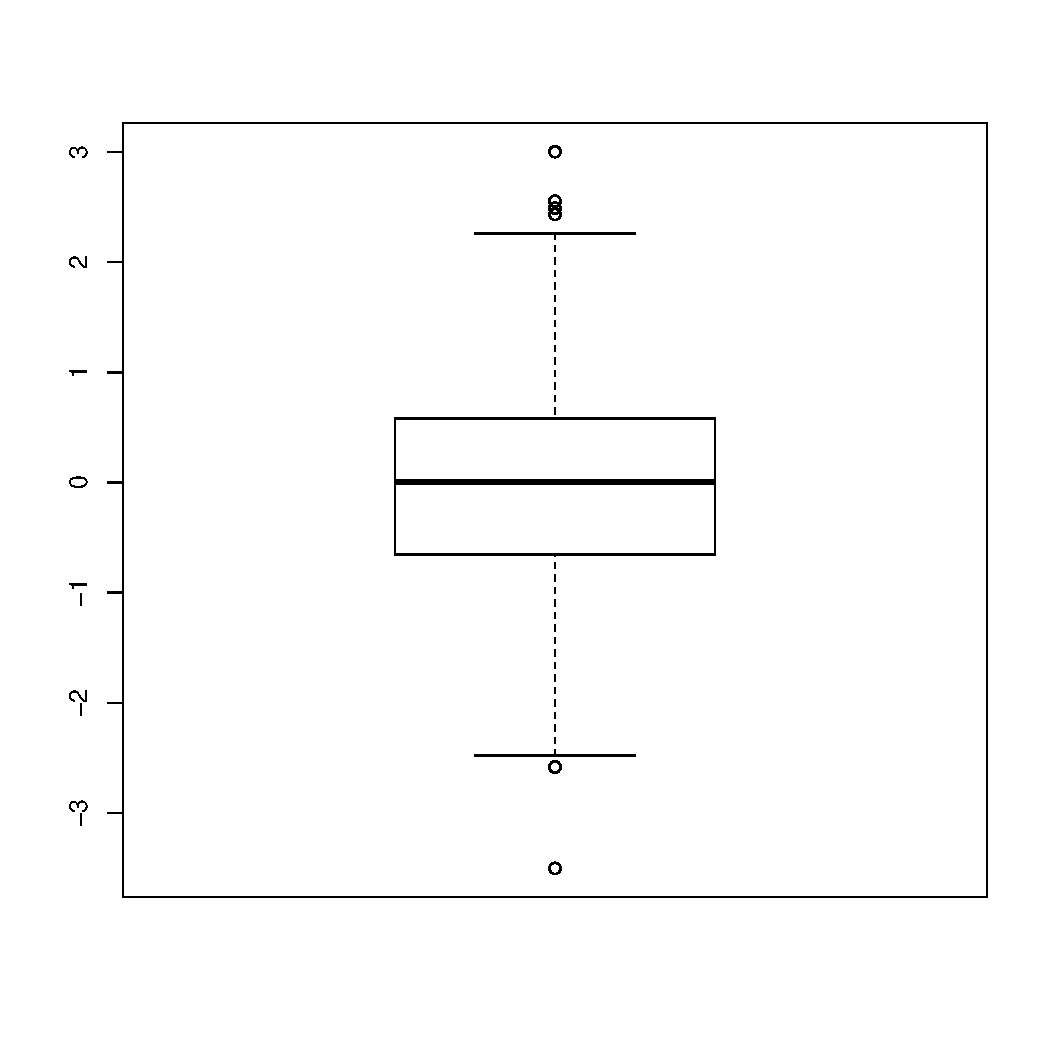
\includegraphics[width=0.7\textwidth]{plots/data.pdf}
    \caption{Een benadering van het boxplot van een normaalverdeling.}
    \label{fig:boxplot_norm}
\end{figure}

\subsection{Locatie schaalfamilie}
\paragraph{Locatie-schaalfamilie} Gegeven een stochastische grootheid \(X\) met verdelingsfunctie \(F\), dan heeft de stochast \(Y=a+bX\) de verdelingsfunctie \(F_{a,b}\) gegeven door
\[
    F_{a,b}(y)=\p(a+bX\leq y)=F\left(\frac{y-a}{b}\right).
\]
De familie kansverdelingen \(\{F_{a,b}\colon a\in\r,b>0\}\) heet de locatie-schaalfamilie behorend bij \(F\) of van \(X\).

\paragraph{Kwantielen} Gegeven een stochast \(X\) met verdelingsfunctie \(F\) is het \(\alpha\)-kwantiel (voor \(\alpha\in(0,1)\)) gelijk aan
\[
    F^{-1}(\alpha)=\inf\{x\colon F(x)\geq\alpha\}.
\]

\paragraph{Ordestatistieken} De ordestatistieken van een steekproef \(X_{1},\dots,X_{n}\) worden gegeven door de rij \(X_{(1)},\dots,X_{(n)}\) zodat ze geplaatst zijn in stijgende volgorde.

Voor de \(i\)-de ordestatistiek geldt dat \(\e F(X_{(i)})=\frac{i}{n+1}\) en algemener geldt dat \(X_{(i)}=a+bF^{-1}\left(\frac{i}{n+1}\right)\) voor \(X_{1},\dots,X_{n}\) elementen verdeeld met \(F_{a,b}\).

\paragraph{QQ-plot} Een QQ-plot van de data \(x_{1},\dots,x_{n}\) ten opzichte van een verdelingsfunctie \(F\) is een grafiek van de punten
\[
    \left\{\left(F^{-1}\left(\frac{i}{n+1}\right),x_{(i)}\right)\mid i=1,\dots,n\right\}.
\]

\subsection{Samenhang}
\paragraph{Scatterplot} Een scatterplot van tweedimensionale data \((x_{1},y_{1}),\dots,(x_{n},y_{n})\) is een grafiek van deze punten in het \(\r^{2}\)-vlak.

\paragraph{Steekproefcorrelatiecoëfficiënt} Het steekproefcorrelatiecoëfficiënt van een steekproef bestaande uit paren \((X_{1},Y_{1}),\dots,(X_{n},Y_{n})\) is
\[
    r_{X,Y}=\frac{\sum_{i=1}^{n}(X_{i}-\avg{X})(Y_{i}-\avg{Y})}{(n-1)\sqrt{S_{X}^{2}}\sqrt{S_{Y}^{2}}}.
\]

Het steekproefcorrelatiecoëfficiënt is een mate van lineairiteit van het verband tussen de waarden \(x_{i}\) en \(y_{i}\).

\paragraph{Auto-correlaties} Gegeven de uitkomst van een steekproef \(x_{1},\dots,x_{n}\) is het auto-correlatiecoëfficiënt een maat van correlatie tussen \(x_{i}\) en \(X_{i-h}\). Het wordt gegeven door
\[
    r_{x}(h)=\frac{\sum_{i=1}^{n-h}(x_{i+h}-\avg{x})(x_{i}-\avg{x})}{(n-h)s_{x}^{2}}.
\]
\section{Schatters}
\subsection{Eigenschappen van schatters}
\paragraph{Wat is een schatter} Een schatter of statistiek is een stochastische vector \(T(X)\) die alleen van \(X\) afhangt.

Als een kansverdeling van \(X\) afhangt van een parameter \(\theta\) zodat \(P_{\theta}\) de kansverdeling is van \(X\), dan is \(\theta\) vaak onbekend, dus dan worden schatters gebruikt om gegeven een realisatie van \(X\) de parameter \(\theta\) te schatten.

\paragraph{Mean Square Error} Gegeven een schatter \(T\) voor een de waarde van \(g(\theta)\), dan is de verwachte kwadratische fout van een schatter de waarde
\[
    \mse(\theta;T)=\e_{\theta}\left\|T-g(\theta)\right\|^{2}.
\]

De Mean Square Error kan ontbonden worden in twee termen:
\[
    \mse(\theta;T)=\var_{\theta}(T)+(\e T-g(\theta))^{2}.
\]

\paragraph{Niet-toelaatbare schatters} Gegeven twee schatters \(T_{1},T_{2}\) van een parameter \(\theta\) met voor elke \(\theta\in\Theta\), met \(\Theta\) de parameterruimte.
\[
    \e_{\theta}\left\|T_{1}-g(\theta)\right\|^{2}\leq\e_{\theta}\left\|T_{2}-g(\theta)\right\|^{2},
\]
dan heet \(T_{2}\) ontoelaatbaar.

\paragraph{Zuivere schatters} Gegeven een schatter \(T\) voor \(g(\theta)\), dan is de onzuiverheid van \(T\) gedefiniëerd als
\[
    \e_{\theta}(T)-g(\theta)=0.
\]
Een schatter is zuiver als voor elke \(\theta\in\Theta\) dat de onzuiverheid gelijk is aan \(0\).

\subsection{Maxmimum Likelihood-Schatters}
\paragraph{Likelihood-functie} Zij \(X\) een stochastische vector met een kansdichtheid \(p_{\theta}\) die afhangt van \(\theta\in\Theta\) met \(\Theta\) de parameterruimte. Dan is voor een vaste \(x\), de functie
\[
    \theta\mapsto L(\theta;x)=p_{\theta}(x),
\]
de likelihood-functie.

\paragraph{Maximum likelihood-schatter} Gegeven een likelihood-functie \(L\) voor een stochast \(X\), dan is de maximum likelihood-schatter \(T(X)\) de waarde voor \(\theta\) zodat \(p_{\theta}(x)\) maximaal is.

\subsection{Momentschatters}
\paragraph{Momenten van een stochast} Gegeven een stochastische variabele afhankelijk van een parameter \(\theta\), dan is het \(j\)-de moment het getal \(\e_{\theta}(X^{j})\), als deze verwachting bestaat.

\paragraph{Steekproefmoment} Gegeven een steekproef \(X_{1},\dots,X_{n}\), dan is het \(j\)-de steekproef moment gegeven door \(\avg{X^{j}}\).

\paragraph{Momentenschatter} Zij \(X_{1},\dots,X_{n}\) een steekproef met onbekende parameter \(\theta\). Dan is de momentschatter de waarde \(\hat{\theta}\) zodat \(\e_{\hat{\theta}}(X^{j})=\avg{X^{j}}\) voor de eerste \(n\) momenten zodat \(\hat{\theta}\) uniek bepaald is. Dat betekent in de praktijk vaak dat \(\hat{\theta}\) bepaald wordt door het eerste moment dat afhankelijk is van de parameter \(\theta\).

\subsection{Bayes-schatters}
Een bayes schatter is een schatter voor een parameter \(\theta\in\Theta\). Er wordt een a priori\footnote{Letterlijk van tevoren.} kansverdeling \(\pi\colon\Theta\to\r\) opgesteld voor \(\theta\), die aangeeft hoe waarschijnlijk een bepaalde waarde van een parameter is. Afhankelijk van de data wordt dan de kansverdeling aangepast tot een a posteriori\footnote{Letterlijk van later, beter vertaald als afgeleid uit de feiten.} kansverdeling.

\paragraph{Bayes-risico} Gegeven een a priori verdeling \(\pi\) is het Bayes-risico van een schatter \(T\) voor \(g(\theta)\) gedefiniëerd als
\[
    R(\theta;T)-\int\e_{\theta}\left(T-g(\theta)\right)^{2}\pi(\theta)\,d\theta.
\]

\paragraph{Bayes-schatter} Gegeven een a priori dichtheid \(\pi\) is de Bayes-schatter de schatter \(T\) die \(R(\theta;T)\) minimaliseert.

De expliciete formule voor de Bayes-schatter is
\[
    T(x)=\frac{\int g(\theta)p_{\theta}(x)\pi(\theta\,dx)}{\int p_{\vartheta}(x)\pi(\vartheta)\,d\vartheta}.
\]
In Bayesiaanse notatie wordt dit geschreven als
\[
    T(x)=\e\left(g\left(\overline{\Theta}\right)\mid X=x\right).
\]

\paragraph{A posteriori dichtheid} De a posteriori dichtheid van \(\overline{\Theta}\) is gelijk aan
\[
    p_{\overline{\Theta}\mid X=x}(\theta)=\frac{p_{\theta}(x)\pi(\theta)}{\int p_{\vartheta}(x)\pi(\vartheta)\,d\vartheta}.
\]
\section{Differentiatie en integratie}

\subsection{Afgeleides}

\paragraph{Wat is de afgeleide?} Een functie $f:\mathbb{R}\to\mathbb{R}$ is differentieerbaar dan en slechts dan als de limiet $\lim{x}{a}\frac{f(x)-f(a)}{x-a}$ bestaat en eindig is. De waarde van de limiet is dan de afgeleide op dat punt. Op elk punt $a$ waar $f$ differentieerbaar is, is $f'(a)$ gedefinieerd als $\lim{x}{a}\frac{f(x)-f(a)}{x-a}$.

\subparagraph{Het domein van $f'$} Omdat $\text{dom}(f')$ de verzameling punten is waarop $f$ differentieerbaar is, geldt dat $\text{dom}(f')\subseteq\text{dom}(f)$.

\paragraph{Afgeleides en continuïteit} Als een functie differentieerbaar is op een punt $a$, dan is de functie ook continu. \textit{Het bewijs hiervoor staat op pagina $225$}.

\paragraph{Eigenschappen van de afgeleide} Zij $f$ en $g$ differentieerbare functies op een punt $a$, dan gelden de volgende stellingen:

\subparagraph{Het bepalen van de afgeleide} Om de afgeleide te bepalen zijn de volgende regels. \textit{Het bewijs hiervoor staat op pagina $226-227$}.


\begin{enumerate}
  \setlength\itemsep{0em}
  \item $(cf)'(a)=c\cdot f'(a)$
  \item $(f+g)'(a)=f'(a)+g'(a)$
  \item Voor het vermenigvuldigen van functies is de productregel: $(fg)'(a)=f'(a)g(a)+f(a)g'(a)$
  \item Voor het berekenen van het quotient van twee functies is de quotientregel: als $f(a)\neq0$, dan geldt dat $(\frac{f}{g})'(a)=\frac{g(a)f'(a)-g'(a)f(a)}{g^{2}(a)}$
\end{enumerate}

\subparagraph{Kettingregel} Zij $f$ een op $a$ differentieerbare functie en $g$ op $f(a)$, dan geldt dat de samengestelde functie $g\circ f$ differentieerbaar is op $a$ en als afgeleide heeft het $(f\circ g)'(a) = g'(f(x))f'(a)$.


\section{Exponenten en logaritmes}
\paragraph{Logaritme base $e$} De functie $\text{log}:\mathbb{R}_{>0}\to\mathbb{R}$ is gedefiniëerd als volgt: $\text{log}(x)\defeq\int_{1}^{x}\frac{1}{t}dt$. Dit is zo gedefiniëerd omdat we \bq weten\eq dat de afgeleide van $\text{log}(x)$ de functie $\frac{1}{x}$ moet zijn en de waarde van het logaritme op $1$ moet $0$ zijn. We schrijven hier voor de logaritme in plaats van $\text{log}$ de functie $L$, maar deze zijn identiek.

\subparagraph{Eigenschappen van de logaritme} De logaritme heeft bepaalde eigenschappen:

  \begin{itemize}
    \setlength\itemsep{0em}
    \item Voor elke $y,z\in\mathbb{R}_{>0}$ geldt dat $\text{log}(yz)=\text{log}(y)+\text{log}(z)$
    \item Voor elke $y,z\in\mathbb{R}_{>0}$ geldt dat $\text{log}(\frac{y}{z})=\text{log}(y)-\text{log}(z)$
    \item De limieten van de logaritme hebben de volgende waarden: $\liminfty{x}\text{log}(x)=\infty$ en $\downlim{x}{0}\text{log}(x)=-\infty$.
  \end{itemize}

\paragraph{E-machten} De functie $e^{x}$ is gedefiniëerd als de inverse van $L(x)$ en we definiëren ook $e=\defeq e^{1}$. We schrijven voor de exponent $E(x)$ in plaats van $e^{x}$.

\subparagraph{Eigenschappen van de e-macht} Ook de $e$-macht heeft bepaalde eigenschappen:

\begin{itemize}
  \setlength\itemsep{0em}
  \item De functie $E$ is strict stijgend, continu en differentiëerbaar op heel $\mathbb{R}$ en $E'=E$
  \item Voor elke $u,v\in\mathbb{R}$ geldt dat $E(u+v)=E(u)E(v)$
  \item De limieten van $E$ zijn als volgt: $\liminfty{x}E(x)=\infty$ en $\limneginfty{x}E(x)=0$
\end{itemize}

\paragraph{Willekeurige machten} Zij $b\in\mathbb{R}_{>0}$. Dan geldt de volgende definitie: $b^{x}\defeq E(xL(b))$. Dan geldt dat $e^{x}=E(xL(e))=E(x)$, dat klopt dus.

\subparagraph{Eigenschappen van willekeurige machten} De volgende eigenschappen zijn waar over willekeurige machten:

\begin{itemize}
  \setlength\itemsep{0em}
  \item De functie $b^{x}$ is continu en differentiëerbaar op heel $\mathbb{R}$
  \item Als $b>0$, dan geldt dat $b^{x}$ strict stijg. Als $b<0$, dan daalt $b^{x}$ strict.
  \item Als $b\neq1$, dan bereikt $b^{x}$ heel $\mathbb{R}_{>0}$
  \item Voor elke $u,v\in\mathbb{R}$ geldt dat $b^{u+v}=b^{u}n^{v}$
\end{itemize}

\paragraph{Logaritme met willekeurige base} De functie $\text{log}_{b}$ is gedefiniëerd als de inverse van de functie $b^{x}$ als $b\neq1$ en $b>0$.

\subparagraph{Eigenschappen van de logaritme met willekeurige base} De functie $\text{log}_{b}$ heeft verscheidene eigenschappen:

\begin{itemize}
  \setlength\itemsep{0em}
  \item De functie $\text{log}_{b}$ is continu en differentiëerbaar op heel $\mathbb{R}_{>0}$
  \item Als $b>1$, dan is $\text{log}_{b}$ strict stijgend. Als $b<1$, dan is $\text{log}_{b}$ strict dalend
  \item Voor alle $y,z\in\mathbb{R}_{>0}$ geldt dat $\text{log}_{b}(yz)=\text{log}_{b}(y)+\text{log}_{b}(z)$
  \item Voor alle $y,z\in\mathbb{R}_{>0}$ geldt dat $\text{log}_{b}(\frac{y}{z})=\text{log}_{b}(y)-\text{log}_{b}(z)$
\end{itemize}

\secnewpage{Appendices}

\subsection{Appendix A: Product van twee rijen}
\label{sec:AA}
\paragraph{Te bewijzen} Zij $s_{n},t_{n}\in\mathbb{R}$. Als $\liminfty{n}(s_{n})=s$ en $\liminfty{n}(t_{n})=t$ dan geldt dat $\liminfty{n}(s_{n}t_{n})=st$.

\begin{proof}
Zij $\epsilon>0$. Omdat $s_{n}$ convergeert is er een $M>0$ zodat $|s_{n}|<M$ voor elke $n\in\mathbb{N}$.\bigskip

\noindent Omdat $\liminfty{n}(t_{n})=t$ is er een $N_{1}$ zodat $|t_{n}-t|<\frac{\epsilon}{2M}$. Dit is omdat ook $\frac{\epsilon}{2M}>0$ en $|t_{n}-t|$ kan willekeurig klein worden, dus ook kleiner dan $\frac{\epsilon}{2M}$. \bigskip

\noindent Ook weten we dat er een $N_{2}$ is zodat $|s_{n}-s|<\frac{\epsilon}{2(|t|+1)}$. De redenering daarvoor is hetzelfde als de redenering voor $t_{n}$. \bigskip

\noindent Laat nu $N=\text{max}\{N_{1},N_{2}\}$. Dan geldt dat als $n>N$ dan zowel $|t_{n}-t|<\frac{\epsilon}{2M}$ als $|s_{n}-s|<\frac{\epsilon}{2(|t|+1)}$ als $n>N$.\bigskip

\noindent We weten dat $|t_{n}-t|<\frac{\epsilon}{2M}$. Daarom geldt ook dat $|s_{n}||t_{n}-t|\leq|s_{n}|\cdot\frac{\epsilon}{2M}$. Merk op dat \bq$\leq$\eq niet omgedraaid wordt omdat $|s_{n}|\geq0$. En omdat $|s_{n}|<M$ voor elke $n$ ($M$ is een bovengrens), geldt dat $|s_{n}|\cdot\frac{\epsilon}{2M}<M\cdot\frac{\epsilon}{2M}=\frac{\epsilon}{2}$ dus ook dat $|s_{n}||t_{n}-t|<\frac{\epsilon}{2}$.\bigskip

\noindent Ook weten we dat $|s_{n}-s|<\frac{\epsilon}{2(|t|+1)}$, waaruit volgt dat $|t||s_{n}-s|<|t|\cdot\frac{\epsilon}{2(|t|+1)}$. Omdat $\frac{\epsilon}{2(|t|+1)}>\frac{\epsilon}{2(|t|)}$ geldt dat $|t||s_{n}-s|<|t|\cdot\frac{\epsilon}{2(|t|)}$ dus dat $|t||s_{n}-s|<\frac{\epsilon}{2}$.\bigskip

\noindent Omdat $|s_{n}||t_{n}-t|<\frac{\epsilon}{2}$ en $|t||s_{n}-s|<\frac{\epsilon}{2}$ geldt ook dat $|s_{n}||t_{n}-t|+|t||s_{n}-s|<\frac{\epsilon}{2}+\frac{\epsilon}{2}=\epsilon$. \bigskip

\noindent Uit stellingen over het vermenigvuldigen van absolute waarden volgt\\ $|s_{n}||t_{n}-t|+|t||s_{n}-s|=|s_{n}t_{n}-s_{n}t|+|s_{n}t-st|$. Dus $|s_{n}t_{n}-s_{n}t|+|s_{n}t-st|<\epsilon$. Volgens de driehoeks-ongelijkheid geldt dan $|s_{n}t_{n}-s_{n}t+s_{n}t-st|\leq|s_{n}t_{n}-s_{n}t|+|s_{n}t-st|$. \bigskip

\noindent Omdat $|s_{n}t_{n}-s_{n}t+s_{n}t-st|=|s_{n}t_{n}-st|$ en $|s_{n}t_{n}-s_{n}t|+|s_{n}t-st|<\epsilon$ geldt dat $|s_{n}t_{n}-st|<\epsilon$ als $n>N$ met $N=\text{max}(N_{1},N_{2})$. \bigskip

\noindent We hebben nu dus bewezen dat voor elke $\epsilon>0$ er een $N$ bestaat, namelijk $\text{max}(N_{1},N_{2})$, zodat voor elke $n>N$ geldt dat $|s_{n}t_{n}-st|<\epsilon$. Dit is wat we moesten bewijzen.

\end{proof}
\subsecnewpage{Appendix B: Cauchy en convergentie}
\label{sec:AB}

\paragraph{Te bewijzen} Een rij $s_{n}\in\sequenceset$. De rij $s_{n}$ convergeert dan en slechts dan als $s_{n}$ Cauchy is. \bigskip

\noindent Voor dit bewijs tonen we aan dat een Cauchy rij convergeert, het bewijs de andere kant op is gegeven in een andere stelling.

\paragraph{Bewijs dat een Cauchy rij convergeert}

\begin{proof}[\unskip\nopunct]

Zij $s_{n}\in\sequenceset$ en $s_{n}$ is Cauchy. Dan geldt dus dat er voor elke $\epsilon>0$ een $N$ bestaat zodat voor elke $m,n>N$ geldt dat $|s_{n}-s_{m}|<\epsilon$. \bigskip

\noindent Omdat $|s_{n}-s_{m}|<\epsilon$ waar is, is ook $-\epsilon<s_{n}-s_{m}<\epsilon$ waar, dus $s_{n}<s_{m}+\epsilon$. Dus is $s_{m}+\epsilon$ een bovengrens voor de verzameling $\{s_{n}:n>N\}$. \bigskip

\noindent Omdat $\{s_{n}:n>N\}$ een bovengrens heeft heeft het dus ook een supremum, namelijk $\text{sup}\{s_{n}:n>N\}$, we noemen dit supremum $v_{N}$. \bigskip

\noindent Het supremum is altijd de kleinste bovengrens van een verzameling dus $v_{N} \leq s_{m}+\epsilon$. Maar dan geldt ook dat $v_{N} - \epsilon \leq s_{m}$, dus $v_{N} - \epsilon$ is een ondergrens van $s_{m}$. Dus geldt dat $s_{m}$ ook een infimum heeft, namelijk $v_{N}-\epsilon$. \bigskip

\noindent Omdat het infimum de kleinste bovengrens is geldt dat $v_{N}-\epsilon\leq\text{inf}\{s_{m}:m>N\}$. We noemen dit infimum $u_{N}$. Dus $v_{N} \leq u_{N}+\epsilon$. \bigskip

\noindent Omdat $\limsup(s_{n})\leq\text{sup}\{s_{n}:n>N\}$ en $\liminf(s_{n})+\epsilon\geq\text{inf}\{s_{n}:n>N\}+\epsilon$ weten we dat $\limsup(s_{n})\leq\text{sup}\{s_{n}:n>N\}\leq\text{inf}\{s_{n}:n>N\}+\epsilon\leq\liminf(s_{n})+\epsilon$. \bigskip

\noindent We hebben nu dus bewezen dat $\limsup(s_{n})\leq\liminf(s_{n})+\epsilon$ voor een willekeurige $\epsilon>0$ als $s_{n}$ Cauchy is. Dus $\limsup(s_{n})=\liminf(s_{n})$. \bigskip

\noindent We weten dat $\liminf(s_{n})\leq\limsup(s_{n})$ en $\limsup(s_{n})\leq\liminf(s_{n})$, dus moet wel gelden dat $\liminf(s_{n})=\limsup(s_{n})$. \bigskip

\noindent Definieer nu $s$ als volgt $s\defeq\limsup{s_{n}}=\liminf{s_{n}}$. Omdat $\liminf{s_{n}}=\limsup{s_{n}}$ waar is, geldt ook dat $\liminfty{n}(s_{n})=s$, dus $s_{n}$ convergeert naar $s$. \bigskip

\noindent We hebben nu dus bewezen dat als een rij $s_{n}$ Cauchy is,dat $s_{n}$ dan ook convergeert.

\end{proof}
\subsecnewpage{Appendix C: Bolzano-Weierstrass}
\label{sec:AC}
Deze appendix bevat twee bewijzen: namelijk dat elke rij een monotone deelrij heeft ($1$), en dat elke begrensde rij een convergente deelrij heeft ($2$).

\paragraph{Bewijs van 1}

\begin{proof}[\unskip\nopunct]

Zij $s_{n}\in\sequenceset$. De $n^{e}$ term van de rij is dominant als voor elke $m>n$ geldt dat $s_{m}<s_{n}$. \bigskip

\noindent Er zijn nu twee verschillende mogelijkheden:

\begin{enumerate}
    \setlength\itemsep{0em}
    \item Er zijn oneindig veel dominante termen.
    \item Er zijn eindig veel dominante termen.
\end{enumerate}

\noindent Als $1$ het geval is, laat dan de functie $(s\circ\sigma)(n)$ de $n^{e}$ dominante tern zijn van $s_{n}$. Dan is de deelrij $(s\circ\sigma)$ dus monotoon dalend, want elke term van $(s\circ\sigma)$ is dominant, dus groter dan alle daaropvolgende termen. \bigskip

\noindent Als $2$ het geval is dan is er dus een laatste dominante term. Oftewel een $N$, waar $s_{N}$ de laatste dominante term is, zodat voor elke $n>N$ geldt dat $s_{n}$ niet dominant is. Dus voor elke $n>N$ is er een $m>n$ zodat $s_{n} \leq s_{m}$. \bigskip

\noindent Kies dan als $n_{1}$ het getal $N+1$. Dan geldt dus dat er een $n_{2}>n_{1}$ is zodat $s_{1} \leq s_{2}$. Ook $s_{n_{2}}$ is niet dominant dus er is een $n_{3}>n_{2}$ zodat $s_{n_{2}} \leq s_{n_{3}}$. Herhaal dit proces tot in het oneindige zodat je een rij krijgt $s_{n_{k}}\in\sequenceset$. Dan geldt voor die rij dat $s_{n_{i}} \leq s_{n_{j}}$ als $i<j$, dus $s_{n_{k}}$ is een monotoon stijgende rij. \bigskip

\noindent We hebben nu bewezen dat in zowel geval $1$ als $2$ de rij $s_{n}$ een monotone deelrij heeft. Dus $s_{n}$ heeft altijd een monotone deelrij. Dit is wat we moesten bewijzen.

\end{proof}

\paragraph{Bewijs van 2}

\begin{proof}[\unskip\nopunct]

Zij $s_{n}\in\sequenceset$ zodat $s_{n}$ begrensd is. We weten dat $s_{n}$ begrensd is, dus elke deelrij van $s_{n}$ is ook begrensd. \bigskip

\noindent Ook weten we dat $s_{n}$ een monotone deelrij $s_{n_{k}}$ heeft, die dus ook begrensd is. De rij $s_{n_{k}}$ is dus een monotone begrensde deelrij, dus $s_{n_{k}}$ convergeert. \bigskip

\noindent Dus elke begrensde rij $s_{n}\in\sequenceset$ heeft een convergente deelrij, namelijk de monotone deelrij $s_{n_{k}}$. Dit is wat we moesten bewijzen.

\end{proof}
\subsecnewpage{Appendix D: Continue functies, minima en maxima}

Zij $f$ een continue functie op het interval $[a,b]$, dan is $f$ een begrensde functie en $f$ neemt haar maximum en minimum aan, dus er zijn een $x_{0},y_{0}\in [a,b]$ zodat voor elke $x\in [a,b]$ geldt dat $f(x_{0}) \leq f(x) \leq f(y_{0})$. We bewijzen eerst dat $f$ begrensd is ($1$) en vervolgens dat $f$ haar maximum en minimum aanneemt ($2$).

\paragraph{Bewijs van 1}

\begin{proof}[\unskip\nopunct]

Stel $f$ is een continue onbegrensde functie is op $[a,b]$, dan geldt voor elke $n\in\mathbb{N}$ dat er een rij $x_{n}\in[a,b]$ bestaat zodat $|f(x_{n}|>n$. \bigskip

\noindent Volgens \hyperref[sec:AC]{Bolzano-Weierstrass} heeft $(x_{n_{k}})$ dan een deelrij die convergeert naar een reëel getal $x_{0}$ omdat $x_{n}$ begrensd is. \bigskip

\noindent Dus $\liminfty{k}(f(x_{n_{k}}))=f(\liminfty{k}(x_{n_{k}})=f(x_{0})$, maar we hebben ook dat $\liminfty{n}(x_{n})=+\infty$ omdat de rij $f(x_{n})$ boven onbegrensd is. \bigskip

\noindent Dit is een tegenspraak, dus moet wel gelden dat $f(x)$ begrensd is.

\end{proof}

\paragraph{Bewijs van 2}

\begin{proof}[\unskip\nopunct]

We weten dat $f(x)$ begrensd is dus er is een $M\defeq\text{sup}\{f(x):x\in[a,b]\}$ die eindig is. \bigskip

\noindent Omdat $M$ het supremum is geldt voor dat voor elke $n\in\mathbb{N}$ er een $y_{n}\in[a,b]$ is zodat $M < \frac{1}{n}<f(y_{n}) \leq M$ omdat $M$ de kleinste bovengrens is. Volgens het \bq Squeeze Lemma\eq geldt dan dat $\liminfty{n}(f(y_{n}))=M$. \bigskip

\noindent Omdat $f(x)$ continu is geldt dat $\liminfty{n}(f(y_{n}))=f(\liminfty{n}(y_{n}))$ en omdat $y_{n}\in[a,b]$ ook $y_{0}\defeq\liminfty{n}(y_{n})\in[a,b]$, dus er is een $y_{0}$ zodat $f$ op $y_{0}$ een maximum aan neent. \bigskip

\noindent We weten dat $-\text{sup}\{-f(x):x\in[a,b]\}=\text{inf}\{f(x):x\in[a,b]\}$. We kunnen op dezelfde manier als hiervoor het supremum van $-f(x)$ bepalen. En dan is er dus ook een $x_{0}$ zodat $-f(x_{0})$ het supremum is van $-f(x)$. En dan is het minimum van $f$ de waarde $f(x_{0})$. \bigskip

\noindent Dus als $f(x)$ continu is op $[a,b]$ neemt deze haar minimum en maximum aan op $[a,b]$. Dit is wat we moesten bewijzen.

\end{proof}
=======
\section{Introductie}

<<<<<<< HEAD
\subsection{De verzameling $\mathbb{R}$}
\paragraph{Algebraïsche eigenschappen}De verzameling breuken $\mathbb{Q}$ heeft de volgende algebraïsche eigenschappen:
\begin{itemize}
    \setlength\itemsep{0em}
    \item[\textbf{A1.}] $a+(b+c)=(a+b)+c$ voor elke $a,b,c\in\mathbb{Q}$.
    \item[\textbf{A2.}] $a+b=b+a$ voor alle $a,b\in\mathbb{Q}$.
    \item[\textbf{A3.}] $a+0=0$ voor alle $a\in\mathbb{Q}$.
    \item[\textbf{A4.}] Voor elke $a\in\mathbb{Q}$ is er een $-a\in\mathbb{Q}$ zodat $a+(-a)=0$
    \item[\textbf{M1.}] $a(bc)=(ab)c$ voor elke $a,b,c\in\mathbb{Q}$.
    \item[\textbf{M2.}] $ab=ba$ voor alle $a,b\in\mathbb{Q}$.
    \item[\textbf{M3.}] $a\cdot1=a$ voor alle $a\in\mathbb{Q}$.
    \item[\textbf{M4.}] Voor elke $a\in\mathbb{Q}$ met $a\neq0$ is er een $a^{-1}\in\mathbb{Q}$ zodat $a \cdot a^{-1} = 1$
\end{itemize}
De eigenschappen \textbf{A1} en \textbf{M1} zijn de \textit{associatieve} eigenschappen van $+$ en $\cdot$ en de eigenschappen \textbf{A2} en \textbf{M2} zijn de \textit{commutatieve} eigenschappen van $+$ en $\cdot$.

\subparagraph{Consequenties van de veld eigenschappen} De volgende eigenschappen volgen uit de algebraïsche eigenschappen van $\mathbb{Q}$:

\begin{enumerate}
    \setlength\itemsep{0em}
    \item Als $a+c=b+c$ dan geldt dat $a=b$.
    \item $a\cdot0=0$ voor alle $a\in\mathbb{Q}$.
    \item $(-a)b=-ab$ voor alle $a,b\in\mathbb{Q}$.
    \item $(-a)(-b)=ab$ voor alle $a,b\in\mathbb{Q}$.
    \item Als $ac=bc$ en $c\neq0$ dan $a=b$.
    \item Als $ab=0$ dan geldt dat $a=0$ of $b=0$.
\end{enumerate}
\textit{De bewijzen van deze stellingen staan op pagina 16 van het boek.}

\paragraph{Ordening}Ook heeft $\mathbb{Q}$ een ordening \bq$\leq$\eq die aan de volgende eigenschappen voldoet:
\begin{itemize}
    \setlength\itemsep{0em}
    \item[\textbf{O1.}] Als $a,b\in\mathbb{Q}$ dan geldt dat $a \leq b$ of $b \leq a$.
    \item[\textbf{O2.}] Als $a \leq b$ en $b \leq a$ dan $a=b$.
    \item[\textbf{O3.}] Als $a \leq b$ en $b \leq c$ dan $a \leq c$.
    \item[\textbf{O4.}] Als $a \leq b$ dan geldt ook dat $a+c \leq b+c$
    \item[\textbf{O5.}] Als $a \leq b$ en $c \geq 0$, dan ook $ac \leq bc$.
\end{itemize}
De eigenschap \textbf{O3} heet de \textit{transitieve} eigenschap. Een veld met een ordening die voldoet aan \textbf{O1} tot en met \textbf{O5} heet een geordend veld.

\subparagraph{Consequenties van de ordening ''$\leq$''}
\begin{enumerate}
    \setlength\itemsep{0em}
    \item Als $a \leq b$ dan $-b \leq -a$.
    \item Als $a \leq b$ en $c\leq0$ dan $bc \leq ac$.
    \item Als $0 \leq a$ en $0 \leq b$ dan $0 \leq ab$.
    \item $0 \leq a^{2}$ voor elke $a\in\mathbb{Q}$.
    \item $0<1$.
    \item Als $0 < a$ dan ook $0 < a^{-1}$.
    \item Als $0<a<b$ dan geldt $0<b^{-1}<a^{-1}$.
\end{enumerate}
\textit{Dit wordt bewezen op pagina 16-17 van het boek.}

\paragraph{Absolute waarde} De absolute waarde is gedefinieerd als volgt:
$$
|a|\defeq
\begin{cases}
    a & \text{als } a\geq 0\\
    -a & \text{als } a<0
\end{cases}
$$
\subparagraph{Stellingen over de absolute waarde} De volgende stellingen over de absolute waarde zijn waar:
\begin{enumerate}
    \setlength\itemsep{0em}
    \item $|a|\geq0$.
    \item $|ab|=|a|\cdot|b|$.
    \item $|a+b|\leq|a|+|b|$.
\end{enumerate}
\textit{Dit wordt bewezen op pagina 17-18 van het boek.}

\paragraph{Afstand} De afstand tussen twee getallen $a,b$ is de $\text{dist}(a,b)$ wat gedefiniëerd is als:
$$\text{dist}(a,b)\defeq|a-b|$$
\paragraph{Stellingen over de afstand} De volgende stelling over afstand is waar:

\subparagraph{Afstand tussen de som van getallen} $\text{dist}(a,c)\leq\text{dist}(a,b)+\text{dist}(b,c)$.

\textit{Dit wordt bewezen op pagina 18 van het boek.}

\paragraph{Stellingen uit opgaven} De volgende handige stellingen worden bewezen in een opgave uit paragraaf $3$:

\subparagraph{Opgave 3.5a} Voor elke $a,b\in\mathbb{R}$ geldt dat $|b| \leq a$ dan en slechts dan als $-a \leq b \leq a$.

\subparagraph{Opgave 3.5b} Voor elke $a,b\in\mathbb{R}$ geldt dat $||b|-|a|| \leq |b-a|$.

\subparagraph{Opgave 3.6b} Laat $a_{1},a_{2},...,a_{n}\in\mathbb{R}$, dan geldt dat $|\sum_{i=1}^{n}a_{i}|\leq\sum_{i=1}^{n}|a_{i}|$
\subsection{De compleetheid van \texorpdfstring{$\mathbb{R}$}{R}}

\paragraph{Maxima en minima} Van een verzameling $S\subseteq\mathbb{R}$ zijn het maximum en minimum als volgt gedefiniëerd:
\subparagraph{Maximum} $s_{0} = \text{max}(S)$ dan en slechts dan als voor elke $s \in S$ geldt dat $s \leq s_{0}$ en $s_{0} \in S$.
\subparagraph{Minimum}$s_{0} = \text{min}(S)$ dan en slechts dan als voor elke $s \in S$ geldt dat $s \geq s_{0}$ en $s_{0} \in S$.

\paragraph{Intervallen} Een interval is een speciaal soort deelverzameling van $\mathbb{R}$, er zijn 4 verschillende intervallen:
\begin{itemize}
    \setlength\itemsep{0em}
    \item $[a,b]\defeq\{x\in\mathbb{R}:a \leq x \leq b\}$ dit heet een gesloten interval. $\text{min}([a,b])=a$ en $\text{max}([a,b])=b$.
    \item $[a,b)\defeq\{x\in\mathbb{R}:a \leq x < b\}$ dit heet een half gesloten interval. $\text{min}([a,b))=a$ en $\text{max}([a,b))$ bestaat niet.
    \item $(a,b]\defeq\{x\in\mathbb{R}:a < x \leq b\}$ dit heet een half gesloten interval. $\text{min}((a,b])=a$ en $\text{max}((a,b])$ bestaat niet.
    \item $(a,b)\defeq\{x\in\mathbb{R}:a < x < b\}$ dit heet een open interval. $\text{min}((a,b))$ bestaat niet en $\text{max}((a,b))$ bestaat niet.
\end{itemize}

\paragraph{Boven- en ondergrenzen} Boven- en ondergrenzen zijn als volgt gedefiniëerd: Laat $S\subseteq\mathbb{R}$ dan geldt

\subparagraph{Bovengrens} Een getal $M$ is een bovengrens van $S$ als voor elke $s \in S$ geldt dat $s \leq M$. Als een verzameling een bovengrens heeft dan heet die verzameling boven begrensd.

\subparagraph{Ondergrens} Een getal $m$ is een ondergrens van $S$ als voor elke $s \in S$ geldt dat $s \geq m$. Als een verzameling een ondergrens heeft dan heet die verzameling onder begrensd.

\paragraph{Stellingen over boven- en ondergrenzen} De volgende stelling wordt gegeven over bovengrenzen:

\subparagraph{Intervallen en begrenzingen} Als $S$ boven en beneden begrensd is, dan zijn er twee getallen $m,M\in\mathbb{R}$ zodat $S\subseteq [m,M]$.

\paragraph{Suprema en infima} Het supremum en infimum van een verzameling zijn als volgt gedefiniëerd:

\subparagraph{Supremum} $M=\text{sup}(S)$ dan en slechts dan als voor elke $s \in S$ geldt dat $s \leq M$ en voor elke $M_{1}<M$ geldt dat er een $s \in S$ is zodat $M_{1}<s$. Dan is $M$ de kleinste bovengrens van $S$.

\subparagraph{Infimum} $m=\text{inf}(S)$ dan en slechts dan als voor elke $s \in S$ geldt dat $m \geq s$ en voor elke $m>m_{1}$ geldt dat er een $s \in S$ waarvoor geldt dat $s<m$. Dan is $m$ de grootste ondergrens van $S$.

\paragraph{Stellingen} In paragraaf 4 van hoofdstuk 1 staan de volgende stellingen:

\subparagraph{Volledigheidsaxioma van $\mathbb{R}$} Het volledigheidsaxioma luidt als volgt: Voor elke $S\subseteq\mathbb{R}$ met $S\neq\emptyset$ met een bovengrens is er een $M\in\mathbb{R}$ zodat $M=\text{sup}(S)$. \textit{Dit is een axioma, er is geen bewijs.}

\subparagraph{``Omgekeerde'' volledigheids \bq axioma\eq} Voor elke $S\in\mathbb{R}$ met $S\neq\emptyset$ met een ondergrens is er een $m\in\mathbb{R}$ zodat $m=\text{inf}(S)$. Het is geen echt axioma want het volgt uit het volledigheidsaxioma. \textit{Het bewijs staat op pagina 24-25 van het boek.}

\subparagraph{Archimedische eigenschap} Zij $a,b\in\mathbb{R}^{+}$ met $a<b$. Dan geldt dat er een $n\in\mathbb{N}$ zodat $na>b$. \textit{Het bewijs staat op pagina 25 van het boek.}

\subparagraph{De dichtheid van $\mathbb{Q}$} Als $a,b\in\mathbb{R}$ en $a<b$ dan is er een $r\in\mathbb{Q}$ zodat $a<r<b$. \textit{Het bewijs staat op pagina 25-26 van het boek.}

\paragraph{Stellingen uit opgaven} De volgende stellingen worden bewezen in een opgave uit paragraaf $4$:

\subparagraph{Opgave 4.7a} Laat $S$ en $T$ verzamelingen zijn met $S,T\subseteq\mathbb{R}$ zodat $S \subseteq T$. Dan geldt dat $\text{inf}(T)\leq\text{inf}(S)\leq\text{sup}(S)\leq\text{sup}(T)$.

\subparagraph{Opgave 4.7b} Laat $S$ en $T$ verzamelingen zijn met met $S,T\subseteq\mathbb{R}$. Dan geldt dat $\text{sup}(S \cup T) = \text{max}\{\text{sup}(S), \text{sup}(T)\}$.

\subparagraph{Opgave 4.8b} Laat $S$ en $T$ verzamelingen zijn zodat voor elke $s \in S$ en $t \in T$ geldt dat $s \leq t$. Dan geldt dat $\text{sup}(S)\leq\text{inf}(T)$.

\subparagraph{Opgave 4.9} Laat $S$ een verzameling zijn zodat $S\subseteq\mathbb{R}$, dan geldt dat $\text{inf}(S)=-\text{sup}(-S)$.

\subparagraph{Opgave 4.14a} Laat $A$ en $B$ verzamelingen zijn met $A,B\subseteq\mathbb{R}$ en $A+B=\{a+b:a \in A \text{ en } b \in B\}$. Dan geldt dat $\text{sup}(A+B)=\text{sup}(A)+\text{sup}(B)$.

\subparagraph{Opgave 4.14b} Laat $A$ en $B$ verzamelingen zijn met $A,B\subseteq\mathbb{R}$. Dan geldt dat $\text{inf}(A+B)=\text{inf}(A)+\text{inf}(B)$.

=======
\subsection{De verzameling $\mathbb{R}$}
\paragraph{Algebraïsche eigenschappen}De verzameling breuken $\mathbb{Q}$ heeft de volgende algebraïsche eigenschappen:
\begin{itemize}
    \setlength\itemsep{0em}
    \item[\textbf{A1.}] $a+(b+c)=(a+b)+c$ voor elke $a,b,c\in\mathbb{Q}$.
    \item[\textbf{A2.}] $a+b=b+a$ voor alle $a,b\in\mathbb{Q}$.
    \item[\textbf{A3.}] $a+0=0$ voor alle $a\in\mathbb{Q}$.
    \item[\textbf{A4.}] Voor elke $a\in\mathbb{Q}$ is er een $-a\in\mathbb{Q}$ zodat $a+(-a)=0$
    \item[\textbf{M1.}] $a(bc)=(ab)c$ voor elke $a,b,c\in\mathbb{Q}$.
    \item[\textbf{M2.}] $ab=ba$ voor alle $a,b\in\mathbb{Q}$.
    \item[\textbf{M3.}] $a\cdot1=a$ voor alle $a\in\mathbb{Q}$.
    \item[\textbf{M4.}] Voor elke $a\in\mathbb{Q}$ met $a\neq0$ is er een $a^{-1}\in\mathbb{Q}$ zodat $a \cdot a^{-1} = 1$
\end{itemize}
De eigenschappen \textbf{A1} en \textbf{M1} zijn de \textit{associatieve} eigenschappen van $+$ en $\cdot$ en de eigenschappen \textbf{A2} en \textbf{M2} zijn de \textit{commutatieve} eigenschappen van $+$ en $\cdot$.

\subparagraph{Consequenties van de veld eigenschappen} De volgende eigenschappen volgen uit de algebraïsche eigenschappen van $\mathbb{Q}$:

\begin{enumerate}
    \setlength\itemsep{0em}
    \item Als $a+c=b+c$ dan geldt dat $a=b$.
    \item $a\cdot0=0$ voor alle $a\in\mathbb{Q}$.
    \item $(-a)b=-ab$ voor alle $a,b\in\mathbb{Q}$.
    \item $(-a)(-b)=ab$ voor alle $a,b\in\mathbb{Q}$.
    \item Als $ac=bc$ en $c\neq0$ dan $a=b$.
    \item Als $ab=0$ dan geldt dat $a=0$ of $b=0$.
\end{enumerate}
\textit{De bewijzen van deze stellingen staan op pagina 16 van het boek.}

\paragraph{Ordening}Ook heeft $\mathbb{Q}$ een ordening \bq$\leq$\eq die aan de volgende eigenschappen voldoet:
\begin{itemize}
    \setlength\itemsep{0em}
    \item[\textbf{O1.}] Als $a,b\in\mathbb{Q}$ dan geldt dat $a \leq b$ of $b \leq a$.
    \item[\textbf{O2.}] Als $a \leq b$ en $b \leq a$ dan $a=b$.
    \item[\textbf{O3.}] Als $a \leq b$ en $b \leq c$ dan $a \leq c$.
    \item[\textbf{O4.}] Als $a \leq b$ dan geldt ook dat $a+c \leq b+c$
    \item[\textbf{O5.}] Als $a \leq b$ en $c \geq 0$, dan ook $ac \leq bc$.
\end{itemize}
De eigenschap \textbf{O3} heet de \textit{transitieve} eigenschap. Een veld met een ordening die voldoet aan \textbf{O1} tot en met \textbf{O5} heet een geordend veld.

\subparagraph{Consequenties van de ordening ''$\leq$''}
\begin{enumerate}
    \setlength\itemsep{0em}
    \item Als $a \leq b$ dan $-b \leq -a$.
    \item Als $a \leq b$ en $c\leq0$ dan $bc \leq ac$.
    \item Als $0 \leq a$ en $0 \leq b$ dan $0 \leq ab$.
    \item $0 \leq a^{2}$ voor elke $a\in\mathbb{Q}$.
    \item $0<1$.
    \item Als $0 < a$ dan ook $0 < a^{-1}$.
    \item Als $0<a<b$ dan geldt $0<b^{-1}<a^{-1}$.
\end{enumerate}
\textit{Dit wordt bewezen op pagina 16-17 van het boek.}

\paragraph{Absolute waarde} De absolute waarde is gedefinieerd als volgt:
$$
|a|\defeq
\begin{cases}
    a & \text{als } a\geq 0\\
    -a & \text{als } a<0
\end{cases}
$$
\subparagraph{Stellingen over de absolute waarde} De volgende stellingen over de absolute waarde zijn waar:
\begin{enumerate}
    \setlength\itemsep{0em}
    \item $|a|\geq0$.
    \item $|ab|=|a|\cdot|b|$.
    \item $|a+b|\leq|a|+|b|$.
\end{enumerate}
\textit{Dit wordt bewezen op pagina 17-18 van het boek.}

\paragraph{Afstand} De afstand tussen twee getallen $a,b$ is de $\text{dist}(a,b)$ wat gedefiniëerd is als:
$$\text{dist}(a,b)\defeq|a-b|$$
\paragraph{Stellingen over de afstand} De volgende stelling over afstand is waar:

\subparagraph{Afstand tussen de som van getallen} $\text{dist}(a,c)\leq\text{dist}(a,b)+\text{dist}(b,c)$.

\textit{Dit wordt bewezen op pagina 18 van het boek.}

\paragraph{Stellingen uit opgaven} De volgende handige stellingen worden bewezen in een opgave uit paragraaf $3$:

\subparagraph{Opgave 3.5a} Voor elke $a,b\in\mathbb{R}$ geldt dat $|b| \leq a$ dan en slechts dan als $-a \leq b \leq a$.

\subparagraph{Opgave 3.5b} Voor elke $a,b\in\mathbb{R}$ geldt dat $||b|-|a|| \leq |b-a|$.

\subparagraph{Opgave 3.6b} Laat $a_{1},a_{2},...,a_{n}\in\mathbb{R}$, dan geldt dat $|\sum_{i=1}^{n}a_{i}|\leq\sum_{i=1}^{n}|a_{i}|$
\subsection{De compleetheid van \texorpdfstring{$\mathbb{R}$}{R}}

\paragraph{Maxima en minima} Van een verzameling $S\subseteq\mathbb{R}$ zijn het maximum en minimum als volgt gedefiniëerd:
\subparagraph{Maximum} $s_{0} = \text{max}(S)$ dan en slechts dan als voor elke $s \in S$ geldt dat $s \leq s_{0}$ en $s_{0} \in S$.
\subparagraph{Minimum}$s_{0} = \text{min}(S)$ dan en slechts dan als voor elke $s \in S$ geldt dat $s \geq s_{0}$ en $s_{0} \in S$.

\paragraph{Intervallen} Een interval is een speciaal soort deelverzameling van $\mathbb{R}$, er zijn 4 verschillende intervallen:
\begin{itemize}
    \setlength\itemsep{0em}
    \item $[a,b]\defeq\{x\in\mathbb{R}:a \leq x \leq b\}$ dit heet een gesloten interval. $\text{min}([a,b])=a$ en $\text{max}([a,b])=b$.
    \item $[a,b)\defeq\{x\in\mathbb{R}:a \leq x < b\}$ dit heet een half gesloten interval. $\text{min}([a,b))=a$ en $\text{max}([a,b))$ bestaat niet.
    \item $(a,b]\defeq\{x\in\mathbb{R}:a < x \leq b\}$ dit heet een half gesloten interval. $\text{min}((a,b])=a$ en $\text{max}((a,b])$ bestaat niet.
    \item $(a,b)\defeq\{x\in\mathbb{R}:a < x < b\}$ dit heet een open interval. $\text{min}((a,b))$ bestaat niet en $\text{max}((a,b))$ bestaat niet.
\end{itemize}

\paragraph{Boven- en ondergrenzen} Boven- en ondergrenzen zijn als volgt gedefiniëerd: Laat $S\subseteq\mathbb{R}$ dan geldt

\subparagraph{Bovengrens} Een getal $M$ is een bovengrens van $S$ als voor elke $s \in S$ geldt dat $s \leq M$. Als een verzameling een bovengrens heeft dan heet die verzameling boven begrensd.

\subparagraph{Ondergrens} Een getal $m$ is een ondergrens van $S$ als voor elke $s \in S$ geldt dat $s \geq m$. Als een verzameling een ondergrens heeft dan heet die verzameling onder begrensd.

\paragraph{Stellingen over boven- en ondergrenzen} De volgende stelling wordt gegeven over bovengrenzen:

\subparagraph{Intervallen en begrenzingen} Als $S$ boven en beneden begrensd is, dan zijn er twee getallen $m,M\in\mathbb{R}$ zodat $S\subseteq [m,M]$.

\paragraph{Suprema en infima} Het supremum en infimum van een verzameling zijn als volgt gedefiniëerd:

\subparagraph{Supremum} $M=\text{sup}(S)$ dan en slechts dan als voor elke $s \in S$ geldt dat $s \leq M$ en voor elke $M_{1}<M$ geldt dat er een $s \in S$ is zodat $M_{1}<s$. Dan is $M$ de kleinste bovengrens van $S$.

\subparagraph{Infimum} $m=\text{inf}(S)$ dan en slechts dan als voor elke $s \in S$ geldt dat $m \geq s$ en voor elke $m>m_{1}$ geldt dat er een $s \in S$ waarvoor geldt dat $s<m$. Dan is $m$ de grootste ondergrens van $S$.

\paragraph{Stellingen} In paragraaf 4 van hoofdstuk 1 staan de volgende stellingen:

\subparagraph{Volledigheidsaxioma van $\mathbb{R}$} Het volledigheidsaxioma luidt als volgt: Voor elke $S\subseteq\mathbb{R}$ met $S\neq\emptyset$ met een bovengrens is er een $M\in\mathbb{R}$ zodat $M=\text{sup}(S)$. \textit{Dit is een axioma, er is geen bewijs.}

\subparagraph{``Omgekeerde'' volledigheids \bq axioma\eq} Voor elke $S\in\mathbb{R}$ met $S\neq\emptyset$ met een ondergrens is er een $m\in\mathbb{R}$ zodat $m=\text{inf}(S)$. Het is geen echt axioma want het volgt uit het volledigheidsaxioma. \textit{Het bewijs staat op pagina 24-25 van het boek.}

\subparagraph{Archimedische eigenschap} Zij $a,b\in\mathbb{R}^{+}$ met $a<b$. Dan geldt dat er een $n\in\mathbb{N}$ zodat $na>b$. \textit{Het bewijs staat op pagina 25 van het boek.}

\subparagraph{De dichtheid van $\mathbb{Q}$} Als $a,b\in\mathbb{R}$ en $a<b$ dan is er een $r\in\mathbb{Q}$ zodat $a<r<b$. \textit{Het bewijs staat op pagina 25-26 van het boek.}

\paragraph{Stellingen uit opgaven} De volgende stellingen worden bewezen in een opgave uit paragraaf $4$:

\subparagraph{Opgave 4.7a} Laat $S$ en $T$ verzamelingen zijn met $S,T\subseteq\mathbb{R}$ zodat $S \subseteq T$. Dan geldt dat $\text{inf}(T)\leq\text{inf}(S)\leq\text{sup}(S)\leq\text{sup}(T)$.

\subparagraph{Opgave 4.7b} Laat $S$ en $T$ verzamelingen zijn met met $S,T\subseteq\mathbb{R}$. Dan geldt dat $\text{sup}(S \cup T) = \text{max}\{\text{sup}(S), \text{sup}(T)\}$.

\subparagraph{Opgave 4.8b} Laat $S$ en $T$ verzamelingen zijn zodat voor elke $s \in S$ en $t \in T$ geldt dat $s \leq t$. Dan geldt dat $\text{sup}(S)\leq\text{inf}(T)$.

\subparagraph{Opgave 4.9} Laat $S$ een verzameling zijn zodat $S\subseteq\mathbb{R}$, dan geldt dat $\text{inf}(S)=-\text{sup}(-S)$.

\subparagraph{Opgave 4.14a} Laat $A$ en $B$ verzamelingen zijn met $A,B\subseteq\mathbb{R}$ en $A+B=\{a+b:a \in A \text{ en } b \in B\}$. Dan geldt dat $\text{sup}(A+B)=\text{sup}(A)+\text{sup}(B)$.

\subparagraph{Opgave 4.14b} Laat $A$ en $B$ verzamelingen zijn met $A,B\subseteq\mathbb{R}$. Dan geldt dat $\text{inf}(A+B)=\text{inf}(A)+\text{inf}(B)$.

>>>>>>> 41d8c4ccd1df145e9b394c4ee2d5ea58fd90f71e

\section{Verdelingsonderzoek}
\subsection{Univariate steekproeven}
\paragraph{Steekproefgemiddelde} Het steekproefgemiddelde van een steekproef \(X_{1},\dots,X_{n}\) is de stochastische grootheid
\[
    \avg{X}=\frac{1}{n}\sum_{i=1}^{n}X_{i}.
\]

\paragraph{Steekproefvariantie} De steekproefvariantie van een steekproef \(X_{1},\dots,X_{n}\) is de stochastische grootheid
\[
    S_{X}^{2}=\frac{1}{n-1}\sum_{i=1}^{n}\left(X_{i}-\avg{X}\right)^{2}.
\]

\subsection{Histogrammen}
Zij \(X_{1},\dots,X_{n}\) een steekproef met bereik \(R\subseteq\r\) en \(a_{0}<\dots<a_{m}\) een partitie van \(R\). Dan is het histogram van de steekproef op een interval \((a_{j-1},a_{j}]\) gegeven door
\[
    h(x)=\frac{1}{a_{j}-a_{j-1}}\sum_{i=1}^{n}1_{(a_{j-1},a_{j}]}(x_{i}).
\]
Het geschaalde histogram schaalt het histogram met een factor \(\frac{1}{n}\). Het geschaalde histogram is dus gelijk aan
\[
    h(x)=\frac{1}{n(a_{j}-a_{j-1})}\sum_{i=1}^{n}1_{(a_{j-1},a_{j}]}(x_{i}).
\]

\subsection{Boxplots}
\paragraph{Kwartielen} Gegeven een steekproef \(X_{1},\dots,X_{n}\) is net \(n\)-de kwartiel de waarde \(X_{i}\) zodat precies \(\frac{n}{4}\) uitkomsten van de steekproef kleiner zijn dan \(X_{i}\).

\paragraph{Boxplots} Een boxplot is een grafiek waarin de kwartielen van een steekproef weergegeven zijn. Het boxplot van een normaalverdeling ziet er bij benadering uit als in figuur \ref{fig:boxplot_norm}.

\begin{figure}[ht]
    \centering
    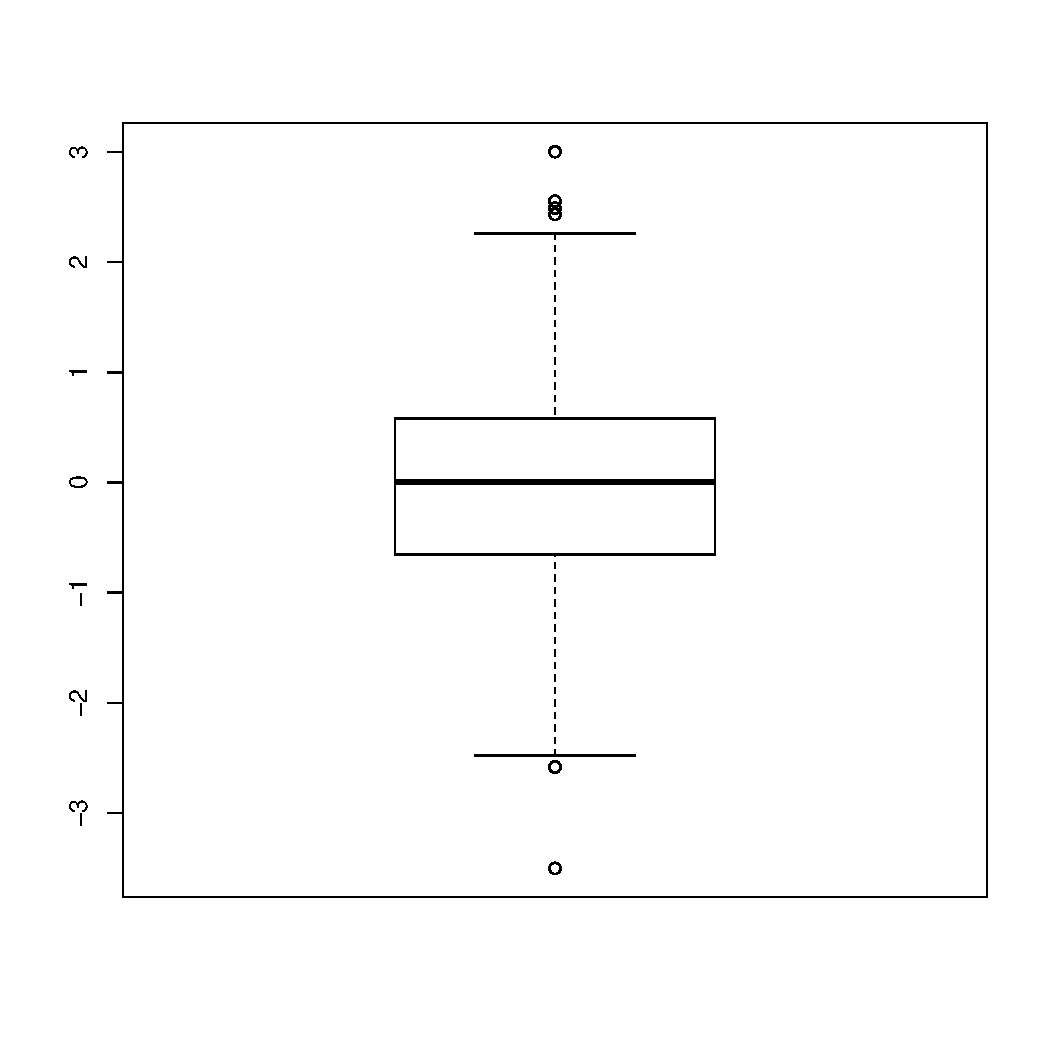
\includegraphics[width=0.7\textwidth]{plots/data.pdf}
    \caption{Een benadering van het boxplot van een normaalverdeling.}
    \label{fig:boxplot_norm}
\end{figure}

\subsection{Locatie schaalfamilie}
\paragraph{Locatie-schaalfamilie} Gegeven een stochastische grootheid \(X\) met verdelingsfunctie \(F\), dan heeft de stochast \(Y=a+bX\) de verdelingsfunctie \(F_{a,b}\) gegeven door
\[
    F_{a,b}(y)=\p(a+bX\leq y)=F\left(\frac{y-a}{b}\right).
\]
De familie kansverdelingen \(\{F_{a,b}\colon a\in\r,b>0\}\) heet de locatie-schaalfamilie behorend bij \(F\) of van \(X\).

\paragraph{Kwantielen} Gegeven een stochast \(X\) met verdelingsfunctie \(F\) is het \(\alpha\)-kwantiel (voor \(\alpha\in(0,1)\)) gelijk aan
\[
    F^{-1}(\alpha)=\inf\{x\colon F(x)\geq\alpha\}.
\]

\paragraph{Ordestatistieken} De ordestatistieken van een steekproef \(X_{1},\dots,X_{n}\) worden gegeven door de rij \(X_{(1)},\dots,X_{(n)}\) zodat ze geplaatst zijn in stijgende volgorde.

Voor de \(i\)-de ordestatistiek geldt dat \(\e F(X_{(i)})=\frac{i}{n+1}\) en algemener geldt dat \(X_{(i)}=a+bF^{-1}\left(\frac{i}{n+1}\right)\) voor \(X_{1},\dots,X_{n}\) elementen verdeeld met \(F_{a,b}\).

\paragraph{QQ-plot} Een QQ-plot van de data \(x_{1},\dots,x_{n}\) ten opzichte van een verdelingsfunctie \(F\) is een grafiek van de punten
\[
    \left\{\left(F^{-1}\left(\frac{i}{n+1}\right),x_{(i)}\right)\mid i=1,\dots,n\right\}.
\]

\subsection{Samenhang}
\paragraph{Scatterplot} Een scatterplot van tweedimensionale data \((x_{1},y_{1}),\dots,(x_{n},y_{n})\) is een grafiek van deze punten in het \(\r^{2}\)-vlak.

\paragraph{Steekproefcorrelatiecoëfficiënt} Het steekproefcorrelatiecoëfficiënt van een steekproef bestaande uit paren \((X_{1},Y_{1}),\dots,(X_{n},Y_{n})\) is
\[
    r_{X,Y}=\frac{\sum_{i=1}^{n}(X_{i}-\avg{X})(Y_{i}-\avg{Y})}{(n-1)\sqrt{S_{X}^{2}}\sqrt{S_{Y}^{2}}}.
\]

Het steekproefcorrelatiecoëfficiënt is een mate van lineairiteit van het verband tussen de waarden \(x_{i}\) en \(y_{i}\).

\paragraph{Auto-correlaties} Gegeven de uitkomst van een steekproef \(x_{1},\dots,x_{n}\) is het auto-correlatiecoëfficiënt een maat van correlatie tussen \(x_{i}\) en \(X_{i-h}\). Het wordt gegeven door
\[
    r_{x}(h)=\frac{\sum_{i=1}^{n-h}(x_{i+h}-\avg{x})(x_{i}-\avg{x})}{(n-h)s_{x}^{2}}.
\]
\section{Schatters}
\subsection{Eigenschappen van schatters}
\paragraph{Wat is een schatter} Een schatter of statistiek is een stochastische vector \(T(X)\) die alleen van \(X\) afhangt.

Als een kansverdeling van \(X\) afhangt van een parameter \(\theta\) zodat \(P_{\theta}\) de kansverdeling is van \(X\), dan is \(\theta\) vaak onbekend, dus dan worden schatters gebruikt om gegeven een realisatie van \(X\) de parameter \(\theta\) te schatten.

\paragraph{Mean Square Error} Gegeven een schatter \(T\) voor een de waarde van \(g(\theta)\), dan is de verwachte kwadratische fout van een schatter de waarde
\[
    \mse(\theta;T)=\e_{\theta}\left\|T-g(\theta)\right\|^{2}.
\]

De Mean Square Error kan ontbonden worden in twee termen:
\[
    \mse(\theta;T)=\var_{\theta}(T)+(\e T-g(\theta))^{2}.
\]

\paragraph{Niet-toelaatbare schatters} Gegeven twee schatters \(T_{1},T_{2}\) van een parameter \(\theta\) met voor elke \(\theta\in\Theta\), met \(\Theta\) de parameterruimte.
\[
    \e_{\theta}\left\|T_{1}-g(\theta)\right\|^{2}\leq\e_{\theta}\left\|T_{2}-g(\theta)\right\|^{2},
\]
dan heet \(T_{2}\) ontoelaatbaar.

\paragraph{Zuivere schatters} Gegeven een schatter \(T\) voor \(g(\theta)\), dan is de onzuiverheid van \(T\) gedefiniëerd als
\[
    \e_{\theta}(T)-g(\theta)=0.
\]
Een schatter is zuiver als voor elke \(\theta\in\Theta\) dat de onzuiverheid gelijk is aan \(0\).

\subsection{Maxmimum Likelihood-Schatters}
\paragraph{Likelihood-functie} Zij \(X\) een stochastische vector met een kansdichtheid \(p_{\theta}\) die afhangt van \(\theta\in\Theta\) met \(\Theta\) de parameterruimte. Dan is voor een vaste \(x\), de functie
\[
    \theta\mapsto L(\theta;x)=p_{\theta}(x),
\]
de likelihood-functie.

\paragraph{Maximum likelihood-schatter} Gegeven een likelihood-functie \(L\) voor een stochast \(X\), dan is de maximum likelihood-schatter \(T(X)\) de waarde voor \(\theta\) zodat \(p_{\theta}(x)\) maximaal is.

\subsection{Momentschatters}
\paragraph{Momenten van een stochast} Gegeven een stochastische variabele afhankelijk van een parameter \(\theta\), dan is het \(j\)-de moment het getal \(\e_{\theta}(X^{j})\), als deze verwachting bestaat.

\paragraph{Steekproefmoment} Gegeven een steekproef \(X_{1},\dots,X_{n}\), dan is het \(j\)-de steekproef moment gegeven door \(\avg{X^{j}}\).

\paragraph{Momentenschatter} Zij \(X_{1},\dots,X_{n}\) een steekproef met onbekende parameter \(\theta\). Dan is de momentschatter de waarde \(\hat{\theta}\) zodat \(\e_{\hat{\theta}}(X^{j})=\avg{X^{j}}\) voor de eerste \(n\) momenten zodat \(\hat{\theta}\) uniek bepaald is. Dat betekent in de praktijk vaak dat \(\hat{\theta}\) bepaald wordt door het eerste moment dat afhankelijk is van de parameter \(\theta\).

\subsection{Bayes-schatters}
Een bayes schatter is een schatter voor een parameter \(\theta\in\Theta\). Er wordt een a priori\footnote{Letterlijk van tevoren.} kansverdeling \(\pi\colon\Theta\to\r\) opgesteld voor \(\theta\), die aangeeft hoe waarschijnlijk een bepaalde waarde van een parameter is. Afhankelijk van de data wordt dan de kansverdeling aangepast tot een a posteriori\footnote{Letterlijk van later, beter vertaald als afgeleid uit de feiten.} kansverdeling.

\paragraph{Bayes-risico} Gegeven een a priori verdeling \(\pi\) is het Bayes-risico van een schatter \(T\) voor \(g(\theta)\) gedefiniëerd als
\[
    R(\theta;T)-\int\e_{\theta}\left(T-g(\theta)\right)^{2}\pi(\theta)\,d\theta.
\]

\paragraph{Bayes-schatter} Gegeven een a priori dichtheid \(\pi\) is de Bayes-schatter de schatter \(T\) die \(R(\theta;T)\) minimaliseert.

De expliciete formule voor de Bayes-schatter is
\[
    T(x)=\frac{\int g(\theta)p_{\theta}(x)\pi(\theta\,dx)}{\int p_{\vartheta}(x)\pi(\vartheta)\,d\vartheta}.
\]
In Bayesiaanse notatie wordt dit geschreven als
\[
    T(x)=\e\left(g\left(\overline{\Theta}\right)\mid X=x\right).
\]

\paragraph{A posteriori dichtheid} De a posteriori dichtheid van \(\overline{\Theta}\) is gelijk aan
\[
    p_{\overline{\Theta}\mid X=x}(\theta)=\frac{p_{\theta}(x)\pi(\theta)}{\int p_{\vartheta}(x)\pi(\vartheta)\,d\vartheta}.
\]
\secnewpage{Appendices}

\subsection{Appendix A: Product van twee rijen}
\label{sec:AA}
\paragraph{Te bewijzen} Zij $s_{n},t_{n}\in\mathbb{R}$. Als $\liminfty{n}(s_{n})=s$ en $\liminfty{n}(t_{n})=t$ dan geldt dat $\liminfty{n}(s_{n}t_{n})=st$.

\begin{proof}
Zij $\epsilon>0$. Omdat $s_{n}$ convergeert is er een $M>0$ zodat $|s_{n}|<M$ voor elke $n\in\mathbb{N}$.\bigskip

\noindent Omdat $\liminfty{n}(t_{n})=t$ is er een $N_{1}$ zodat $|t_{n}-t|<\frac{\epsilon}{2M}$. Dit is omdat ook $\frac{\epsilon}{2M}>0$ en $|t_{n}-t|$ kan willekeurig klein worden, dus ook kleiner dan $\frac{\epsilon}{2M}$. \bigskip

\noindent Ook weten we dat er een $N_{2}$ is zodat $|s_{n}-s|<\frac{\epsilon}{2(|t|+1)}$. De redenering daarvoor is hetzelfde als de redenering voor $t_{n}$. \bigskip

\noindent Laat nu $N=\text{max}\{N_{1},N_{2}\}$. Dan geldt dat als $n>N$ dan zowel $|t_{n}-t|<\frac{\epsilon}{2M}$ als $|s_{n}-s|<\frac{\epsilon}{2(|t|+1)}$ als $n>N$.\bigskip

\noindent We weten dat $|t_{n}-t|<\frac{\epsilon}{2M}$. Daarom geldt ook dat $|s_{n}||t_{n}-t|\leq|s_{n}|\cdot\frac{\epsilon}{2M}$. Merk op dat \bq$\leq$\eq niet omgedraaid wordt omdat $|s_{n}|\geq0$. En omdat $|s_{n}|<M$ voor elke $n$ ($M$ is een bovengrens), geldt dat $|s_{n}|\cdot\frac{\epsilon}{2M}<M\cdot\frac{\epsilon}{2M}=\frac{\epsilon}{2}$ dus ook dat $|s_{n}||t_{n}-t|<\frac{\epsilon}{2}$.\bigskip

\noindent Ook weten we dat $|s_{n}-s|<\frac{\epsilon}{2(|t|+1)}$, waaruit volgt dat $|t||s_{n}-s|<|t|\cdot\frac{\epsilon}{2(|t|+1)}$. Omdat $\frac{\epsilon}{2(|t|+1)}>\frac{\epsilon}{2(|t|)}$ geldt dat $|t||s_{n}-s|<|t|\cdot\frac{\epsilon}{2(|t|)}$ dus dat $|t||s_{n}-s|<\frac{\epsilon}{2}$.\bigskip

\noindent Omdat $|s_{n}||t_{n}-t|<\frac{\epsilon}{2}$ en $|t||s_{n}-s|<\frac{\epsilon}{2}$ geldt ook dat $|s_{n}||t_{n}-t|+|t||s_{n}-s|<\frac{\epsilon}{2}+\frac{\epsilon}{2}=\epsilon$. \bigskip

\noindent Uit stellingen over het vermenigvuldigen van absolute waarden volgt\\ $|s_{n}||t_{n}-t|+|t||s_{n}-s|=|s_{n}t_{n}-s_{n}t|+|s_{n}t-st|$. Dus $|s_{n}t_{n}-s_{n}t|+|s_{n}t-st|<\epsilon$. Volgens de driehoeks-ongelijkheid geldt dan $|s_{n}t_{n}-s_{n}t+s_{n}t-st|\leq|s_{n}t_{n}-s_{n}t|+|s_{n}t-st|$. \bigskip

\noindent Omdat $|s_{n}t_{n}-s_{n}t+s_{n}t-st|=|s_{n}t_{n}-st|$ en $|s_{n}t_{n}-s_{n}t|+|s_{n}t-st|<\epsilon$ geldt dat $|s_{n}t_{n}-st|<\epsilon$ als $n>N$ met $N=\text{max}(N_{1},N_{2})$. \bigskip

\noindent We hebben nu dus bewezen dat voor elke $\epsilon>0$ er een $N$ bestaat, namelijk $\text{max}(N_{1},N_{2})$, zodat voor elke $n>N$ geldt dat $|s_{n}t_{n}-st|<\epsilon$. Dit is wat we moesten bewijzen.

\end{proof}
\subsecnewpage{Appendix B: Cauchy en convergentie}
\label{sec:AB}

\paragraph{Te bewijzen} Een rij $s_{n}\in\sequenceset$. De rij $s_{n}$ convergeert dan en slechts dan als $s_{n}$ Cauchy is. \bigskip

\noindent Voor dit bewijs tonen we aan dat een Cauchy rij convergeert, het bewijs de andere kant op is gegeven in een andere stelling.

\paragraph{Bewijs dat een Cauchy rij convergeert}

\begin{proof}[\unskip\nopunct]

Zij $s_{n}\in\sequenceset$ en $s_{n}$ is Cauchy. Dan geldt dus dat er voor elke $\epsilon>0$ een $N$ bestaat zodat voor elke $m,n>N$ geldt dat $|s_{n}-s_{m}|<\epsilon$. \bigskip

\noindent Omdat $|s_{n}-s_{m}|<\epsilon$ waar is, is ook $-\epsilon<s_{n}-s_{m}<\epsilon$ waar, dus $s_{n}<s_{m}+\epsilon$. Dus is $s_{m}+\epsilon$ een bovengrens voor de verzameling $\{s_{n}:n>N\}$. \bigskip

\noindent Omdat $\{s_{n}:n>N\}$ een bovengrens heeft heeft het dus ook een supremum, namelijk $\text{sup}\{s_{n}:n>N\}$, we noemen dit supremum $v_{N}$. \bigskip

\noindent Het supremum is altijd de kleinste bovengrens van een verzameling dus $v_{N} \leq s_{m}+\epsilon$. Maar dan geldt ook dat $v_{N} - \epsilon \leq s_{m}$, dus $v_{N} - \epsilon$ is een ondergrens van $s_{m}$. Dus geldt dat $s_{m}$ ook een infimum heeft, namelijk $v_{N}-\epsilon$. \bigskip

\noindent Omdat het infimum de kleinste bovengrens is geldt dat $v_{N}-\epsilon\leq\text{inf}\{s_{m}:m>N\}$. We noemen dit infimum $u_{N}$. Dus $v_{N} \leq u_{N}+\epsilon$. \bigskip

\noindent Omdat $\limsup(s_{n})\leq\text{sup}\{s_{n}:n>N\}$ en $\liminf(s_{n})+\epsilon\geq\text{inf}\{s_{n}:n>N\}+\epsilon$ weten we dat $\limsup(s_{n})\leq\text{sup}\{s_{n}:n>N\}\leq\text{inf}\{s_{n}:n>N\}+\epsilon\leq\liminf(s_{n})+\epsilon$. \bigskip

\noindent We hebben nu dus bewezen dat $\limsup(s_{n})\leq\liminf(s_{n})+\epsilon$ voor een willekeurige $\epsilon>0$ als $s_{n}$ Cauchy is. Dus $\limsup(s_{n})=\liminf(s_{n})$. \bigskip

\noindent We weten dat $\liminf(s_{n})\leq\limsup(s_{n})$ en $\limsup(s_{n})\leq\liminf(s_{n})$, dus moet wel gelden dat $\liminf(s_{n})=\limsup(s_{n})$. \bigskip

\noindent Definieer nu $s$ als volgt $s\defeq\limsup{s_{n}}=\liminf{s_{n}}$. Omdat $\liminf{s_{n}}=\limsup{s_{n}}$ waar is, geldt ook dat $\liminfty{n}(s_{n})=s$, dus $s_{n}$ convergeert naar $s$. \bigskip

\noindent We hebben nu dus bewezen dat als een rij $s_{n}$ Cauchy is,dat $s_{n}$ dan ook convergeert.

\end{proof}
\subsecnewpage{Appendix C: Bolzano-Weierstrass}
\label{sec:AC}
Deze appendix bevat twee bewijzen: namelijk dat elke rij een monotone deelrij heeft ($1$), en dat elke begrensde rij een convergente deelrij heeft ($2$).

\paragraph{Bewijs van 1}

\begin{proof}[\unskip\nopunct]

Zij $s_{n}\in\sequenceset$. De $n^{e}$ term van de rij is dominant als voor elke $m>n$ geldt dat $s_{m}<s_{n}$. \bigskip

\noindent Er zijn nu twee verschillende mogelijkheden:

\begin{enumerate}
    \setlength\itemsep{0em}
    \item Er zijn oneindig veel dominante termen.
    \item Er zijn eindig veel dominante termen.
\end{enumerate}

\noindent Als $1$ het geval is, laat dan de functie $(s\circ\sigma)(n)$ de $n^{e}$ dominante tern zijn van $s_{n}$. Dan is de deelrij $(s\circ\sigma)$ dus monotoon dalend, want elke term van $(s\circ\sigma)$ is dominant, dus groter dan alle daaropvolgende termen. \bigskip

\noindent Als $2$ het geval is dan is er dus een laatste dominante term. Oftewel een $N$, waar $s_{N}$ de laatste dominante term is, zodat voor elke $n>N$ geldt dat $s_{n}$ niet dominant is. Dus voor elke $n>N$ is er een $m>n$ zodat $s_{n} \leq s_{m}$. \bigskip

\noindent Kies dan als $n_{1}$ het getal $N+1$. Dan geldt dus dat er een $n_{2}>n_{1}$ is zodat $s_{1} \leq s_{2}$. Ook $s_{n_{2}}$ is niet dominant dus er is een $n_{3}>n_{2}$ zodat $s_{n_{2}} \leq s_{n_{3}}$. Herhaal dit proces tot in het oneindige zodat je een rij krijgt $s_{n_{k}}\in\sequenceset$. Dan geldt voor die rij dat $s_{n_{i}} \leq s_{n_{j}}$ als $i<j$, dus $s_{n_{k}}$ is een monotoon stijgende rij. \bigskip

\noindent We hebben nu bewezen dat in zowel geval $1$ als $2$ de rij $s_{n}$ een monotone deelrij heeft. Dus $s_{n}$ heeft altijd een monotone deelrij. Dit is wat we moesten bewijzen.

\end{proof}

\paragraph{Bewijs van 2}

\begin{proof}[\unskip\nopunct]

Zij $s_{n}\in\sequenceset$ zodat $s_{n}$ begrensd is. We weten dat $s_{n}$ begrensd is, dus elke deelrij van $s_{n}$ is ook begrensd. \bigskip

\noindent Ook weten we dat $s_{n}$ een monotone deelrij $s_{n_{k}}$ heeft, die dus ook begrensd is. De rij $s_{n_{k}}$ is dus een monotone begrensde deelrij, dus $s_{n_{k}}$ convergeert. \bigskip

\noindent Dus elke begrensde rij $s_{n}\in\sequenceset$ heeft een convergente deelrij, namelijk de monotone deelrij $s_{n_{k}}$. Dit is wat we moesten bewijzen.

\end{proof}
\subsecnewpage{Appendix D: Continue functies, minima en maxima}

Zij $f$ een continue functie op het interval $[a,b]$, dan is $f$ een begrensde functie en $f$ neemt haar maximum en minimum aan, dus er zijn een $x_{0},y_{0}\in [a,b]$ zodat voor elke $x\in [a,b]$ geldt dat $f(x_{0}) \leq f(x) \leq f(y_{0})$. We bewijzen eerst dat $f$ begrensd is ($1$) en vervolgens dat $f$ haar maximum en minimum aanneemt ($2$).

\paragraph{Bewijs van 1}

\begin{proof}[\unskip\nopunct]

Stel $f$ is een continue onbegrensde functie is op $[a,b]$, dan geldt voor elke $n\in\mathbb{N}$ dat er een rij $x_{n}\in[a,b]$ bestaat zodat $|f(x_{n}|>n$. \bigskip

\noindent Volgens \hyperref[sec:AC]{Bolzano-Weierstrass} heeft $(x_{n_{k}})$ dan een deelrij die convergeert naar een reëel getal $x_{0}$ omdat $x_{n}$ begrensd is. \bigskip

\noindent Dus $\liminfty{k}(f(x_{n_{k}}))=f(\liminfty{k}(x_{n_{k}})=f(x_{0})$, maar we hebben ook dat $\liminfty{n}(x_{n})=+\infty$ omdat de rij $f(x_{n})$ boven onbegrensd is. \bigskip

\noindent Dit is een tegenspraak, dus moet wel gelden dat $f(x)$ begrensd is.

\end{proof}

\paragraph{Bewijs van 2}

\begin{proof}[\unskip\nopunct]

We weten dat $f(x)$ begrensd is dus er is een $M\defeq\text{sup}\{f(x):x\in[a,b]\}$ die eindig is. \bigskip

\noindent Omdat $M$ het supremum is geldt voor dat voor elke $n\in\mathbb{N}$ er een $y_{n}\in[a,b]$ is zodat $M < \frac{1}{n}<f(y_{n}) \leq M$ omdat $M$ de kleinste bovengrens is. Volgens het \bq Squeeze Lemma\eq geldt dan dat $\liminfty{n}(f(y_{n}))=M$. \bigskip

\noindent Omdat $f(x)$ continu is geldt dat $\liminfty{n}(f(y_{n}))=f(\liminfty{n}(y_{n}))$ en omdat $y_{n}\in[a,b]$ ook $y_{0}\defeq\liminfty{n}(y_{n})\in[a,b]$, dus er is een $y_{0}$ zodat $f$ op $y_{0}$ een maximum aan neent. \bigskip

\noindent We weten dat $-\text{sup}\{-f(x):x\in[a,b]\}=\text{inf}\{f(x):x\in[a,b]\}$. We kunnen op dezelfde manier als hiervoor het supremum van $-f(x)$ bepalen. En dan is er dus ook een $x_{0}$ zodat $-f(x_{0})$ het supremum is van $-f(x)$. En dan is het minimum van $f$ de waarde $f(x_{0})$. \bigskip

\noindent Dus als $f(x)$ continu is op $[a,b]$ neemt deze haar minimum en maximum aan op $[a,b]$. Dit is wat we moesten bewijzen.

\end{proof}
>>>>>>> 41d8c4ccd1df145e9b394c4ee2d5ea58fd90f71e

\end{document}
